\documentclass[11pt, letterpaper]{article}
\usepackage[margin=0.45in]{geometry}
\setlength{\columnsep}{0.25in}
\usepackage{multicol}
\usepackage{paracol}
\usepackage[english]{babel}
\usepackage{graphicx}
\graphicspath{{Figures/}{./}}
\usepackage{wrapfig}
\usepackage{amsmath}
\usepackage{amssymb}
\usepackage{amsthm}
\usepackage{booktabs}
\usepackage{indentfirst}
\usepackage{siunitx}
\usepackage{mhchem}
\usepackage[justification=centering]{caption}
\usepackage{subfigure}
\usepackage{float}
\usepackage{outlines}
\usepackage{tabularray}
\usepackage{apacite}
\usepackage{url}

% TODO: ensure that everything (other than personal stuff) is third person

\DeclareSIUnit\angstrom{\text {Å}}
\pagenumbering{roman}
\globalcounter{figure}
\globalcounter{table}

\title{IB CHEMISTRY HL IA
\\
Clay Soil Swelling}
\author{}
\date{}

\begin{document}
\nocite{*}

\maketitle

\begin{center}
    Research Question: What is the relationship between
    the factor by which the volume of
    sodium bentonite swells and the concentration of hydrochloric acid (\ce{HCl}) /\unit{mol.dm^{-3}} when the acidic solution and sodium bentonite
    mixes?
    \\
\end{center}

\begin{center}
    Candidate Code:
    \\
    Session: May 2024
    \\
    Page Count: 12
\end{center}
\newpage

\tableofcontents
\newpage

\pagenumbering{arabic}
% \begin{multicols*}{2}

\section{Introduction}

\setcounter{page}{1}

From the engineers in my family, I have always been exposed to ideas
surrounding the various unguessable factors that can
result in the failure of a structure.
While my father was discussing the various
aspects important for consideration in the foundation
of a structure, I was intrigued when he mentioned the different
degrees that clay soils will swell under different acidic conditions,
in which structures that are built upon clay soils must
be engineered to be able to withstand the expansion of the soil
when the soil is contaminated from "natural processes" such
as rain \cite{ramavaraprasadSwellingCharacteristicsSoils2018a}.
While clay soil under an engineering context involves
predicting and designing a structure according to the
type of clay soil and the common levels of acidity
to come into contact with the clay, I was brought to the
research question of "What is the relationship between
the factor by which the volume of
sodium bentonite swells and the concentration of \ce{H+} of an acidic solution /\unit{mol.dm^{-3}} when the acidic solution and sodium bentonite
mixes?"


\section{Background Information}

Clay soils, such as sodium bentonite, are composed of negatively charged
"platelike layers" that are balanced by cations nested in between
those layers \cite{chenClaySwellingRole2022}. Clay swelling when mixed with a solution mainly occurs
as a result of the attraction of water molecules into the interlayer space
of the clay, causing the interlayer space to grow \cite{chenClaySwellingRole2022}.

The effect that the acidity of the solution plays on the degree to which
the clay swells will vary depending on the composition of the clay.
Sodium bentonite is expected to swell less when mixed with higher acidity
solutions due to the interlayer cation replacement
of \ce{Na+} with the \ce{H+} ions made available from
the ionization of hydrochloric acid (\ce{HCl}), in which because the
ionic radius of \ce{H+} (\SI{0.012}{\angstrom})
is lower than that of \ce{Na+} (\SI{1.02}{\angstrom}),
then the amount of clay swelling is reduced \cite{ramavaraprasadSwellingCharacteristicsSoils2018a}.
Despite these values, it is important to investigate the exact relationship
of the clay's factor of swelling as a function of the mixed acid,
in this case hydrochloric acid, as the ionic radii of \ce{Na+}
and \ce{H+} do not make this relationship obvious and
the cited literature regarding clay swelling focus on the
pattern of the clay swelling as time progresses.


\section{Proof of Concept}

Before the experiment was performed, a proof of concept
was done to determine whether there is a difference
in swelling between different concentrations and what the
range of concentrations should be in order to obtain
a holistic result.

Initially, two test trials were done where \SI{1.0}{mL} of
\SI{1.0}{mol.dm^{-3}} \ce{HCl} and \SI{1.0}{mL} of water
were each mixed into \SI{1.0}{mL} of bentonite clay in
\SI{10}{mL} graduated cylinders. In both mixtures, the
bentonite clay was not completely mixed with the solutions,
with virtually all the acidic solution being absorbed by the
clay as seen in Figure \ref*{fig:poc1MHCL}.

This heavy absorption of the clay was heavily problematic
for the actual experiment, as not only does it result in
partial swelling of the clay soil but also leads to difficulty
in cleaning out the mixture especially in a \SI{10}{mL} graduated
cylinder. On the packaging of the bentonite clay, it recommends
that the clay and solution should be mixed at a 1:10 ratio of volume.

Two additional test trials were done with \SI{10}{mL} of
\SI{1.0}{mol.dm^{-3}} \ce{HCl} and \SI{10}{mL} of water,
each mixed into \SI{1.0}{mL} of bentonite clay in
\SI{25}{mL} graduated cylinders. Mixing between
bentonite clay and the solutions improved with a
significant difference in swelling between the two mixtures
(the acid swelled the clay by a factor of about 3, while
the water swelled the clay by a factor of about 5.6).
These two test trials are shown in Figure \ref*{fig:betterPOC}.

It was at this point when there was the realization that it
is likely better to mix the clay into the solution rather than
the other way around to ensure optimal absorption of the solution
by the clay. However, what is to come next is determining the
best maximum \ce{[H+]} to see the optimal holistic result
in the relationship between the factor of swelling and \ce{[H+]}.
In this proof of concept, the method of mixing the solution
into the clay was continued to ensure that there is consistency
between the test trials.

One interesting qualitative observation at this point was that
in the mixture of bentonite clay with water, there was a hole
in the immersed bentonite clay, as seen in Figure \ref*{fig:hole}.

It is unknown why this occurs, but it may be suggested that
this could be as a result of mixing solution into the clay,
therefore mixing clay into the solution may mitigate this issue.

Finally, \SI{10}{mL} of \SI{2.0}{mol.dm^{-3}} was mixed with \SI{1.0}{mL}
of bentonite clay. The factor to which the bentonite had swollen by
in this mixture (2.8 times) doesn't differ much compared to the
mixture with \SI{10}{mL} of \SI{1.0}{mol.dm^{-3}} \ce{HCl}, therefore
it was decided that \SI{1.0}{mol.dm^{-3}} will be the maximum
concentration for this investigation.






\begin{paracol}{3}

    \begin{figure}[H]
        \centering
        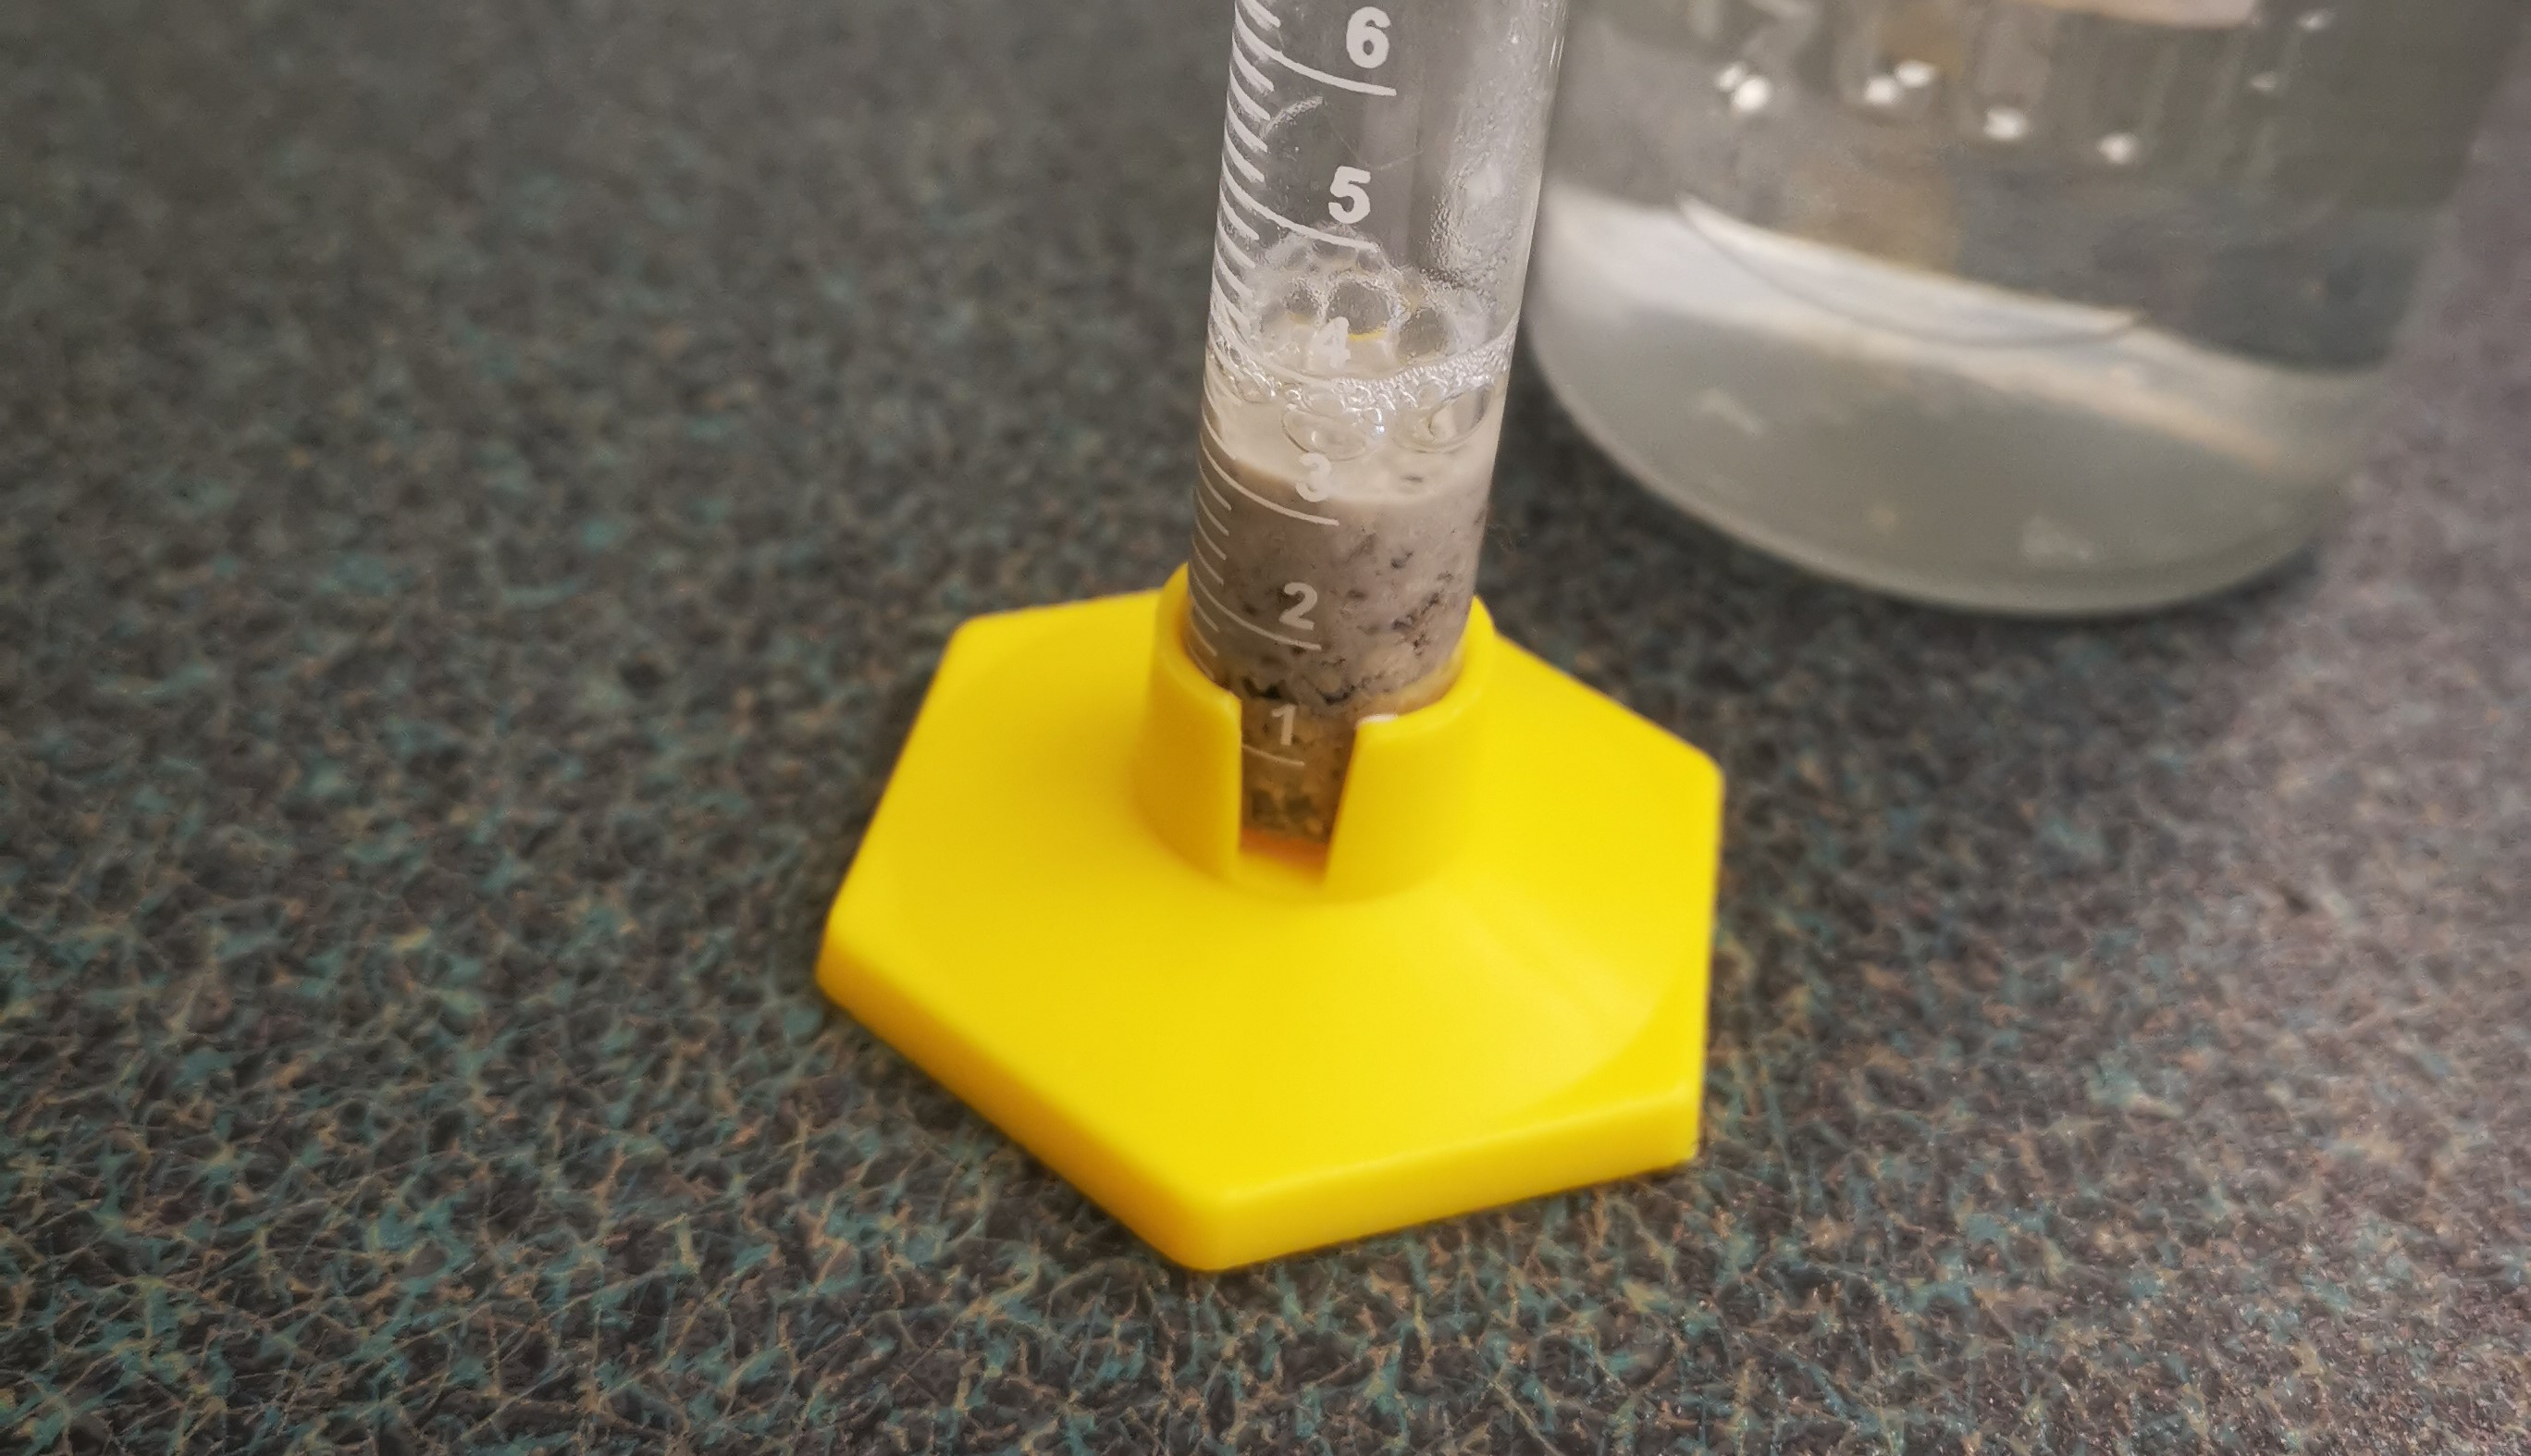
\includegraphics[width=0.28\textwidth]{poc1MHCL.jpg}
        \caption{Proof of Concept Trial of \SI{1.0}{mL} \SI{1.0}{mol.dm^{-3}} \ce{HCl} with \SI{1.0}{mL} bentonite clay}
        \label{fig:poc1MHCL}
    \end{figure}
    \switchcolumn


    \begin{figure}[H]
        \centering
        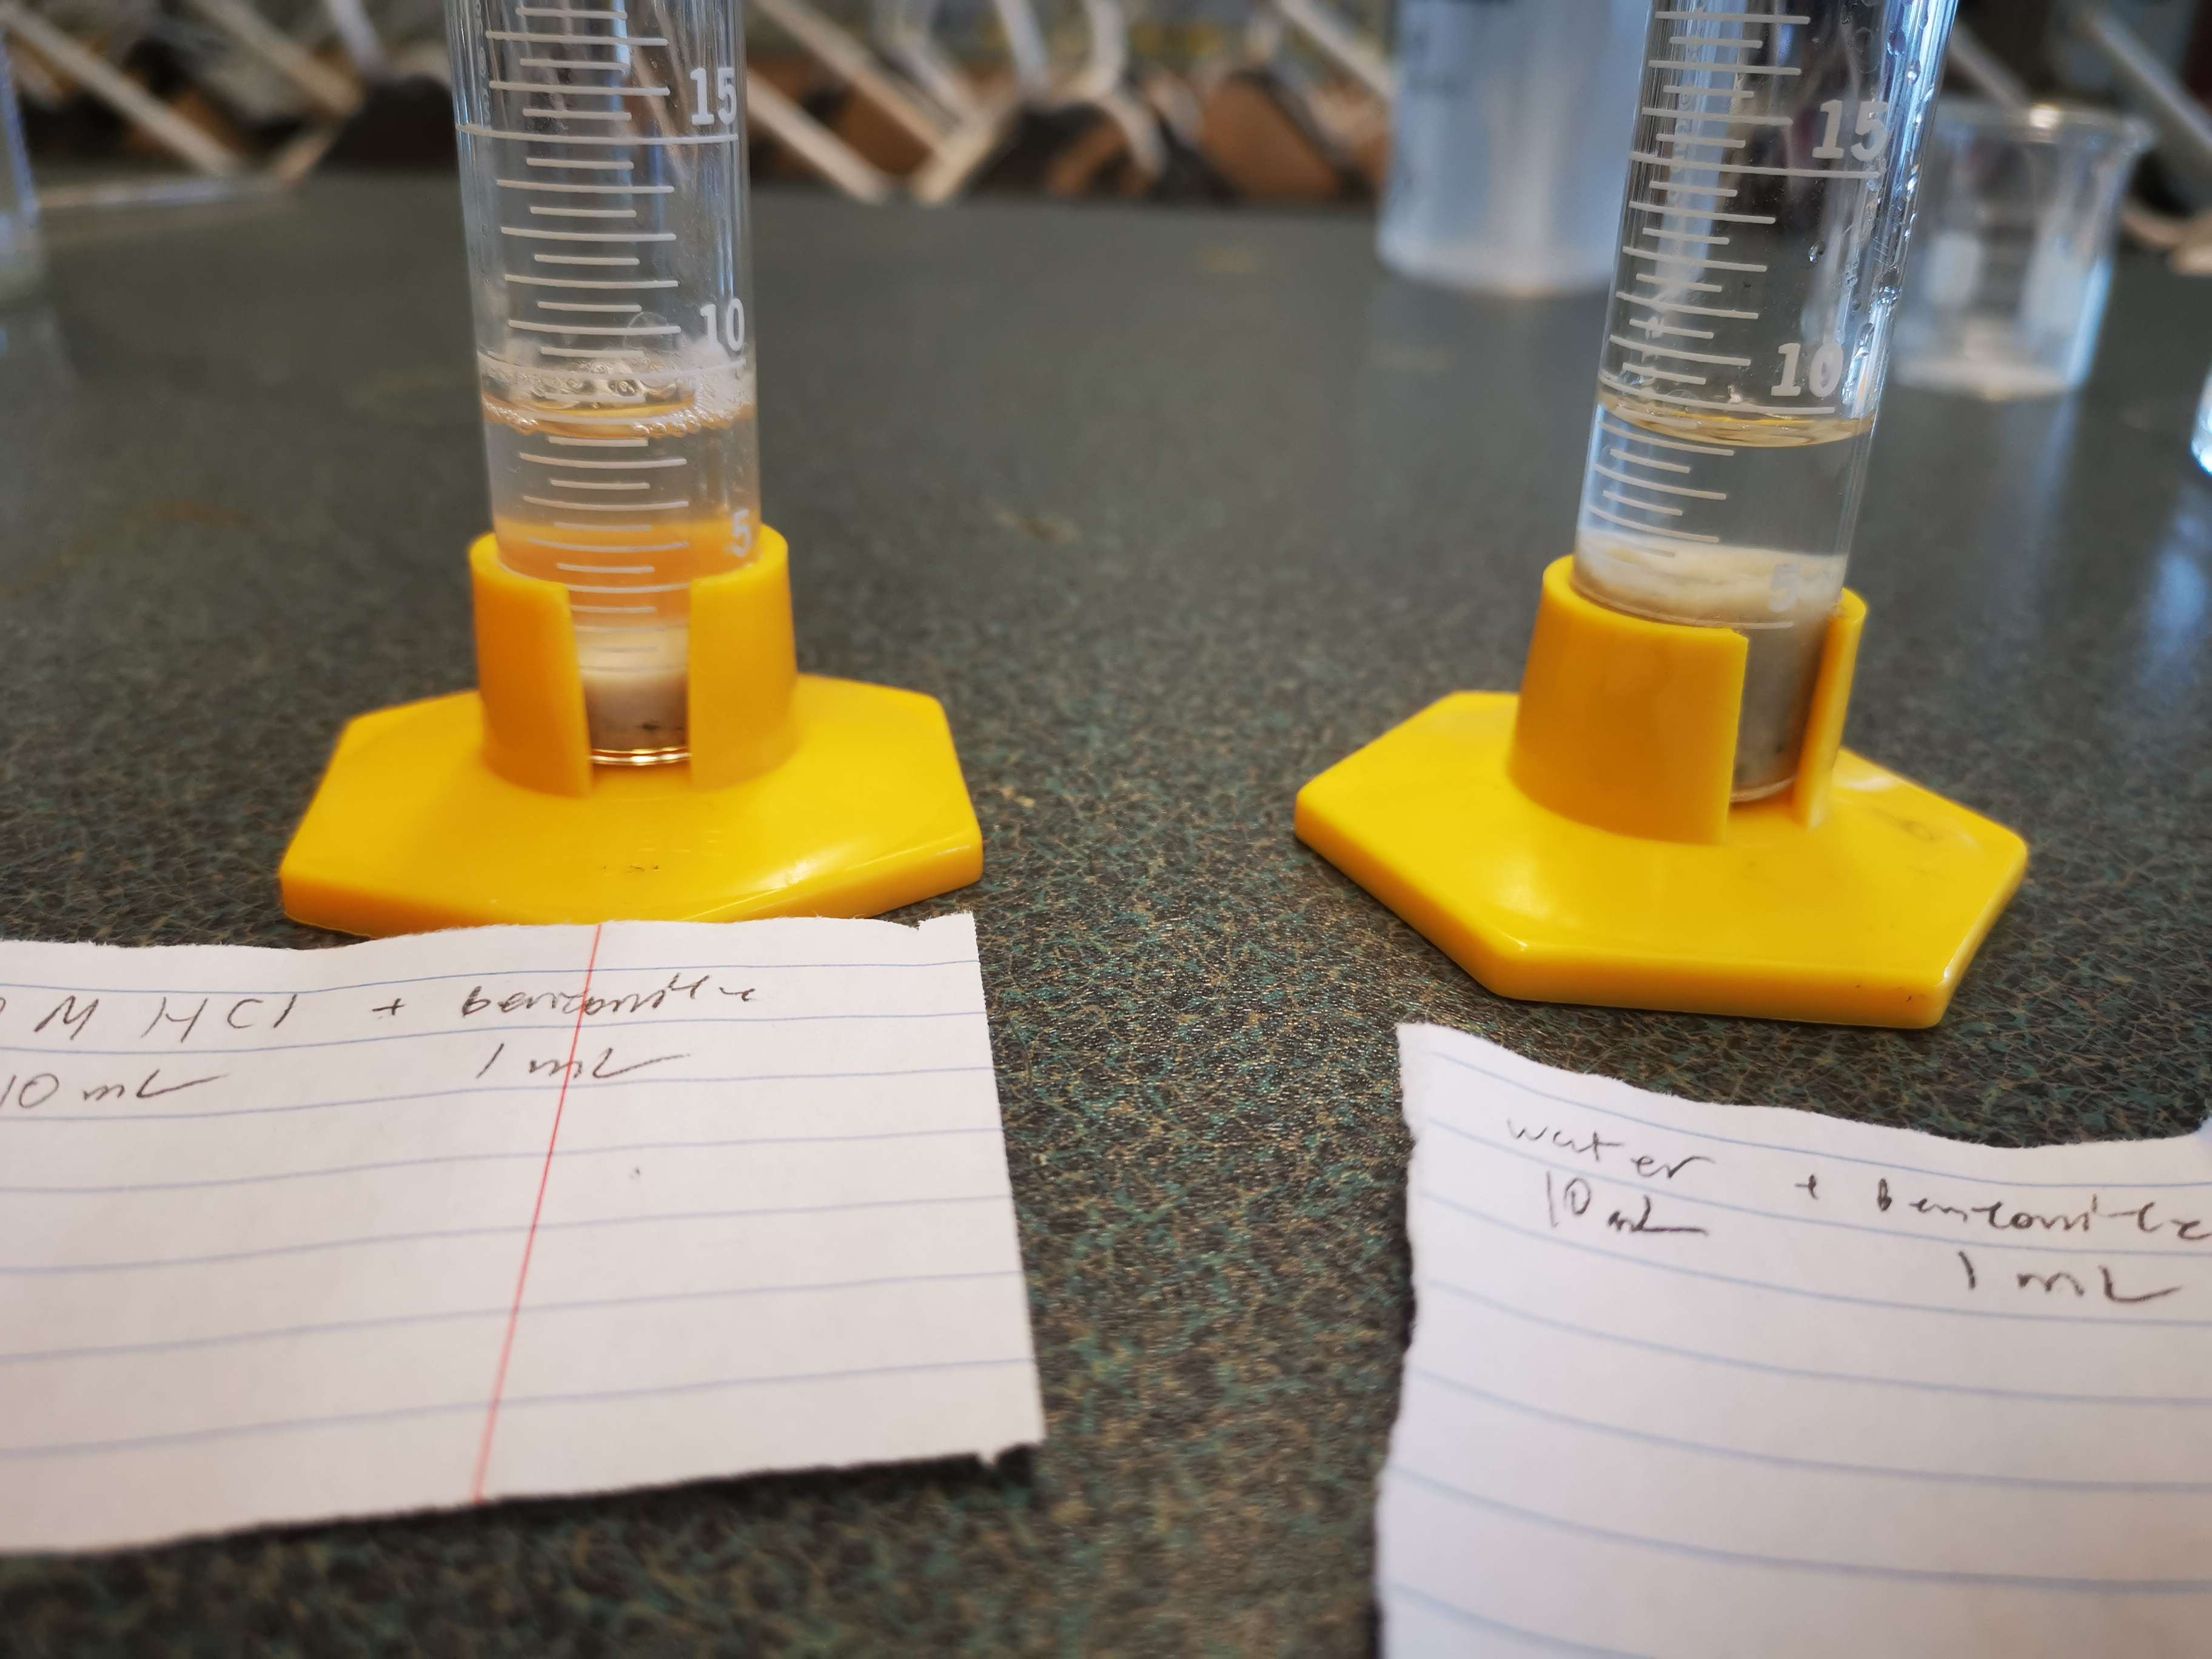
\includegraphics[width=0.28\textwidth]{betterPOC.jpg}
        \caption{Proof of Concept Trial of \SI{10}{mL} \SI{1.0}{mol.dm^{-3}} \ce{HCl} (left) and \SI{10}{mL} of water (right) with \SI{1.0}{mL} bentonite clay}
        \label{fig:betterPOC}
    \end{figure}

    \switchcolumn
    \begin{figure}[H]
        \centering
        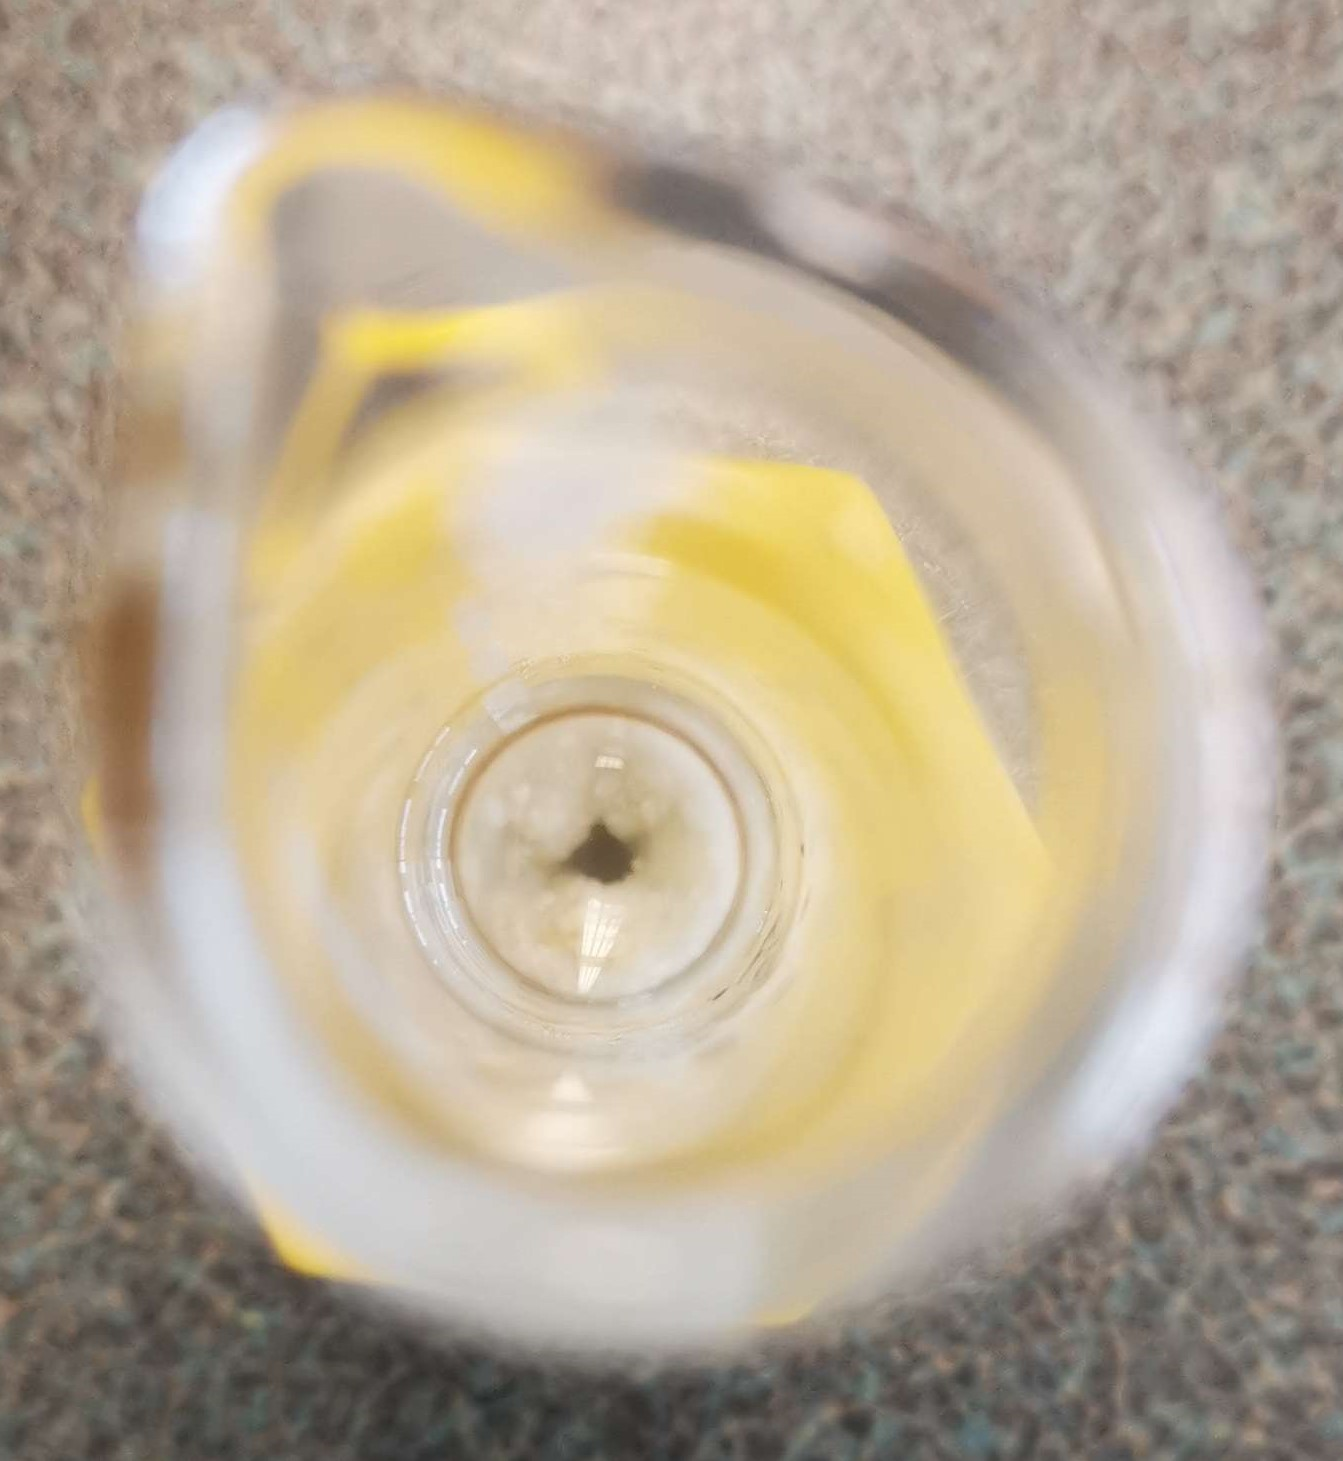
\includegraphics[width=0.18\textwidth]{hole.jpg}
        \caption{Hole in bentonite clay in test trial between \SI{10}{mL} of water with \SI{1.0}{mL} bentonite}
        \label{fig:hole}
    \end{figure}

\end{paracol}

\section{Hypothesis}

The hypothesis for this experiment is that
the factor by which the volume of
sodium bentonite swells will decrease as the concentration of \ce{H+} ions of the mixed
solution increases in a linear fashion
given the prediction that a linear increase in \ce{[H+]} means a linear increase
of the amount of \ce{H+} ions that become available to replace \ce{Na+} ions.

However, it is predicted that there will be a point where
a decrease in swelling will begin to slow down when a deficiency
of \ce{Na+} ions in between the bentonite clay layers grows.
It is hypothesized that this effect will be manifested
as a horizontal asymptote on the plotted graph of the Factor
of swelling as a function of \ce{[H+]}.

\section{Variables}

\begin{paracol}{2}
    \subsection{Independent Variable}
    The manipulated variable is the concentration of the hydrochloric acid solution mixed with the
    bentonite clay /\unit{mol.dm^{-3}}. In this lab, the manipulated variable will be
    changed by acid dilution.
    \switchcolumn
    \subsection{Dependent Variable}
    The responding variable is the factor by which the clay has swollen by.
    The responding variable will be measured using a \SI{25}{mL} graduated cylinder.

\end{paracol}


\begin{paracol}{2}
    \subsection{Controlled Variable 1: Clay swelling duration}
    \subsubsection{How to control it}
    For each trial, set a timer for 10 minutes and record
    the final volume when the timer ends.
    \subsubsection{Why it must be controlled}
    Inconsistent durations of time between trials will entail
    that the clays that were allows more time to swell will be able
    to swell more than it should relative to the other trials.
    Note that in the process, there will be a slight difference in duration
    allowed between the 5 trials that share the same \ce{[H+]}.
    This is not significant as due to the slow nature of clay swelling,
    a difference in duration by under a minute will not lead to
    \switchcolumn
    \subsection{Controlled Variable 2: Volume of solution mixed with clay}
    \subsubsection{How to control it}
    Consistently measure \SI{10.00}{mL} of solution for each trial
    using a \SI{10.00}{mL} pipette.
    \subsubsection{Why it must be controlled}
    Differing the volume of solution mixed with the clay between different
    trials will lead to major difference of the amount \ce{H+} ions available to
    be exchanged with \ce{Na+} ions in the clay. Because this ion
    exchange is essential to the behaviour of swelling in bentonite clay,
    the volume of the solution mixed with the clay must be controlled.
    major inconsistencies.
\end{paracol}

\subsection{Controlled Variable 3: Volume of initial clay}
\subsubsection{How to control it}
Consistently use a set volume of bentonite clay for each trial. Note
that because bentonite is rather sticky and therefore is tough
to clean out of a thin graduated cylinder, then it is best to
standardize the volume of clay committed for the experiment
by taking the volume of the dry bentonite with a graduated cylinder
and transferring it to a weigh boat to determine what mass of clay
is associative with the set volume of clay.
\subsubsection{Why it must be controlled}
Differing the volume of initial clay between trials will lead to
major differences in sodium ions present in the clay. This will
lead to inconsistencies of the swelling factor as there will
be more/less sodium ions ready to be exchanged with
hydrogen ions.



\section{Equipment and Materials}

\begin{multicols}{2}
    % TODO: mention beakers for clay and water
    \begin{itemize}
        \item Lab Apron
        \item Lab Goggles
        \item Waste Beakers
        \item Distilled Water
        \item sodium bentonite clay
        \item \SI{1.00}{mol.dm^{-3}} hydrochloric acid (HCl) \\ (\(\pm\) \SI{0.03}{mol.dm^{-3}})
        \item \SI{0.100}{mol.dm^{-3}} hydrochloric acid (HCl) \\ (\(\pm\) \SI{0.006}{mol.dm^{-3}})
        \item (1) \SI{10.00}{mL} Graduated Cylinder (\(\pm\) \SI{0.02}{mL})
        \item (5) \SI{25.0}{mL} Graduated Cylinders (\(\pm\) \SI{0.3}{mL})
        \item (3) \SI{100.0}{mL} Volumetric Flasks (\(\pm\) \SI{0.2}{mL})
        \item \SI{10.00}{mL} pipette (\(\pm\) \SI{0.04}{mL})
        \item (5) Weigh Boats
        \item Pipette pump
        \item Scoopula
        \item (2) Stir rod
        \item Paper towel
        \item Digital Balance (\(\pm\) \SI{0.003}{g})
        \item Timer
    \end{itemize}

\end{multicols}

\section{Safety, Environmental, and Ethical Considerations}

\begin{paracol}{2}
    \begin{itemize}
        \item A lab apron and eye protection must be worn at all times during the experiment
        \item No consumption of food or water during the experiment
        \item Eyes that have made contact with the hydrochloric acid should be rinsed with water for several minutes, with contact lenses being removed if possible in the middle of the rinsing process.
        \item Thoroughly wash any skin with water and soap if it has been in contact with hydrochloric acid. Hands should also be thoroughly washed after completing the experiment.
        \item Move to an area of fresh air if hydrochloric acid is inhaled.
    \end{itemize}
    \switchcolumn
    \begin{itemize}
        \item If hydrochloric acid is swallowed, rinse mouth. Do not induce vomiting
        \item When performing acid dilution, always add the acid into the water and not the other way around.
        \item Dispose of any waste containing acid to a waste beaker labelled with contents and approximate \ce{[H+]}. Dispose hydrochloric acid by neutralizing it with baking soda and flushing it with water 10 times the original waste volume
        \item Take caution when attaching/detaching a pipette pump onto/from a pipette, ensuring that the distance between your two hands do not apply overwhelming torque onto the pipette
    \end{itemize}
\end{paracol}

\section{Procedure}

% TODO: mention beakers of clay and water
\begin{enumerate}
    \item Put on lab apron and eye protection
    \item Using the \SI{10}{mL} pipette, transfer \SI{50}{mL} of distilled water to the \SI{100}{mL} volumetric flask \label{step:pip}
    \item Top up the \SI{100}{mL} volumetric flask with \SI{1.0}{mol.dm^{-3}} \ce{HCl} to obtain a \SI{100}{mL} solution of \SI{0.5}{mol.dm^{-3}} \ce{HCl} \label{step:mix}
    \item Repeat Steps \ref*{step:pip} and \ref*{step:mix} using \SI{0.1}{mol^{-3}} \ce{HCl} to obtain a \SI{100}{mL} solution of \SI{0.05}{mol.dm^{-3}} \ce{HCl}
    \item Using the \SI{10}{mL} pipette, transfer \SI{10}{mL} of distilled water to the \SI{100}{mL} volumetric flask
    \item Top up the \SI{100}{mL} volumetric flask with \SI{1.0}{mol.dm^{-3}} \ce{HCl} to obtain a \SI{100}{mL} solution of \SI{0.01}{mol.dm^{-3}} \ce{HCl}
    \item Using a scoopula, transfer bentonite clay into the \SI{10}{mL} graduated cylinder until there is \SI{1}{mL} of bentonite clay
    \item Place a weigh boat onto the digital balance and tare the balance
    \item Transfer all the bentonite clay in the \SI{10}{mL} graduated cylinder into the weight boat and record the mass of the bentonite clay \label{step:findClayMass}
    \item \label{step:measureMass} Place another weight boat on the digital balance, tare the balance, then transfer enough bentonite clay using the scoopula such that the mass read by the balance matches the mass found in Step \ref*{step:findClayMass}.
    \item Repeat Step \ref*{step:measureMass} for all 5 weigh boats.
    \item Using the \SI{10}{mL} pipette, transfer \SI{10}{mL} of a solution to each \SI{25}{mL} graduated cylinder
    \item Flick the bottom of each weight boat such that all the clay reaches to one corner, then proceed to transfer the clay of each weigh boat to each \SI{25}{mL} graduated cylinder as quickly as possible
    \item Set a timer for 10 minutes
    \item As the timer approaches its end, start flicking each graduated cylinder to force all the bentonite clay to be submerged at the bottom of the graduated cylinder
    \item Once the timer ends, record the final volumes of bentonite clay in each \SI{25}{mL} graduated cylinder
    \item If the solution is acidic, first transfer remaining solution into the waste beaker, using an acid designated stir rod to remove the majority of the clay. Fill up the graduated cylinder with water, then transfer the water and any large chunks of clay into the waste beaker again
    \item \label{step:clean} Repeatedly fill the graduated cylinder with water and scrub the interior with a stir rod wrapped by paper towel until no clay remains
    \item Repeat Steps \ref*{step:measureMass} to \ref*{step:clean} for all solutions
    \item Wash your hands thoroughly after the experiment and clean the laboratory workspace
\end{enumerate}


\begin{figure}[H]
    \centering
    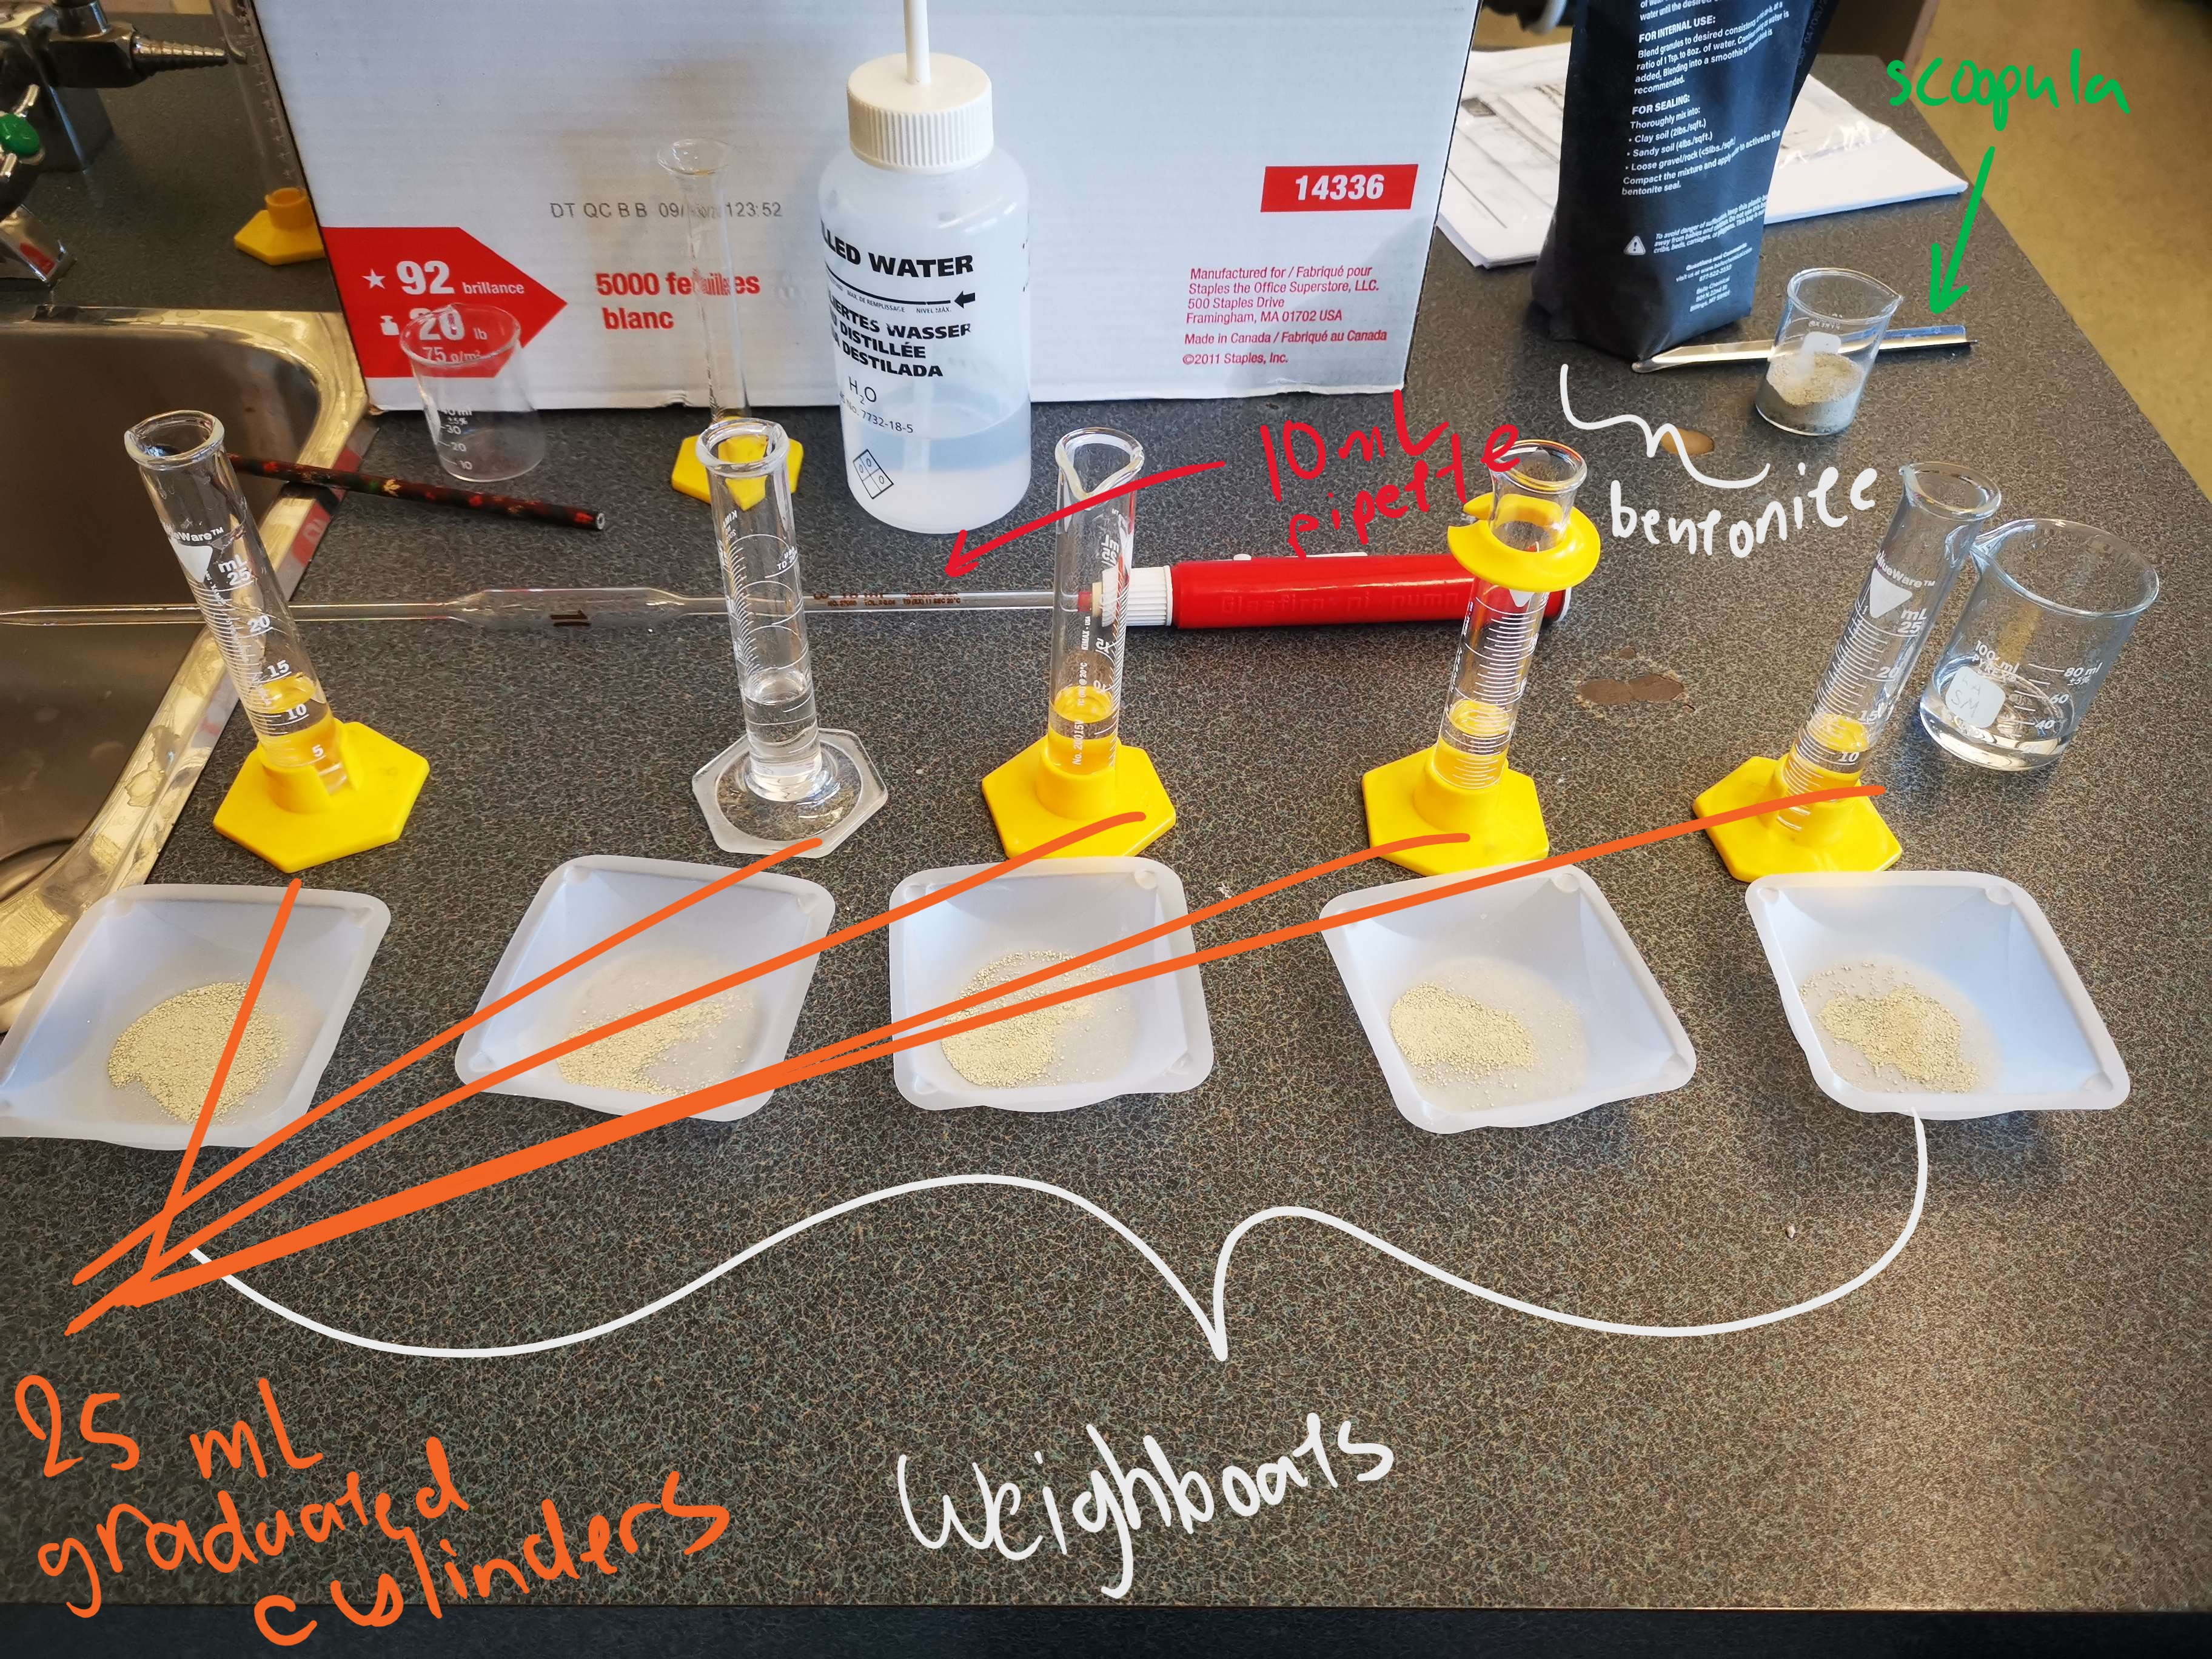
\includegraphics[width=0.5\textwidth]{labSetup.jpg}
    \caption{Lab setup prior to mixing between bentonite clay and the solution}
    \label{fig:labSetup}
\end{figure}

% TODO: additional mini figures
% \begin{minipage}{0.3\textwidth}
% \end{minipage}
% \hfill
% \begin{minipage}{0.3\textwidth}
% \end{minipage}
% \hfill
% \begin{minipage}{0.3\textwidth}
% \end{minipage}

\section{Evidence}
\subsection{Qualitative Observations}
\begin{outline}
    \1 The sodium bentonite clay is a grey powder that appears in various sizes (fine to the size of a grain of sand). Fine parts of the clay easily stick to glassware and the weigh boats
    \1 The hydrochloric acid is a clear colourless solution for all \ce{[H+]} concentrations used in this experiment
    \1 None of the trials lead to a hole in the submerged clay that was observed in the proof of concept mixture between water and bentonite clay
    \1 When the clay is mixed with water
    \2 The submerged clay releases black solids resembling sesame seeds
    \2 The solution immediately changes into a murky white
    \2 The submerged clay turns into a dark grey in the form of fluffy particles signficantly larger than the dry grains of clay
    \1 When the clay is mixed with \SI{0.01}{mol.dm^{-3}} \ce{HCl}
    \2 The clay turns into a dark grey, but not as dark as in the trials with water
    \2 Initially, solution mixed with the clay remains clear and colourless. However, the solution turns white and murky upon agitation
    \1 When the clay is mixed with \SI{0.05}{mol.dm^{-3}} \ce{HCl} or \SI{0.1}{mol.dm^{-3}} \ce{HCl}
    \2 The solution overtime turns from clear and colourless to white and murky
    \2 Submerged clay is whiter than that of the \SI{0.01}{mol.dm^{-3}} trials
    \1 When the clay is mixed with \SI{0.5}{mol.dm^{-3}} \ce{HCl} or \SI{1.0}{mol.dm^{-3}} \ce{HCl}
    \2 The solution immediately turns white and murky
    \2 There is bubbling at the meniscus of the solution
    \2 All the submerged clay is fine and does not stick to the glassware
    \1 Especially for trials when \(\ce{[HCl]} = \SI{1.00}{mol.dm^{-3}}\), the final volume of the submerged bentonite clay sometimes was below the minimum graduation on the \SI{25}{mL} graduated cylinder. Therefore, the volume of the bentonite clay was difficult to determine in these trials.
\end{outline}

\subsection{Quantitative Data}

\begin{itemize}
    \item The initial volume of the bentonite clay was \(\SI{1.00}{mL} \pm \SI{0.02}{mL}\). This initial volume was standardized to be \(\SI{0.810}{g} \pm \SI{0.003}{g}\).
\end{itemize}

\begin{table}[H]
    \fontsize{9pt}{9pt}\selectfont
    \centering
    \caption{Raw data of final volume of bentonite clay for 5 trials of each hydrochloric acid concentration}
    \begin{tblr}{
        cells = {c},
        cell{1}{1} = {r=2}{},
        cell{1}{2} = {c=5}{},
        vlines,
        hline{1,3-9} = {-}{},
                hline{2} = {2-6}{},
            }
        Concentration of \ce{HCl} in the solution /$\unit{mol.dm^{-3}}$ & Final Volume of submerged bentonite clay /$\unit{mL} \pm \SI{0.3}{mL}$ &         &         &         &         \\
                                                                        & Trial 1                                                                & Trial 2 & Trial 3 & Trial 4 & Trial 5 \\
        0 (Distilled Water)                                             & 8.5                                                                    & 8.5     & 7.5     & 9.0     & 8.0     \\
        $0.0100 \pm 0.0007$                                             & 8.0                                                                    & 8.5     & 9.0     & 9.5     & 7.5     \\
        $0.050 \pm 0.003$                                               & 5.5                                                                    & 5.5     & 5.5     & 6.0     & 5.0     \\
        $0.100 \pm 0.006$                                               & 5.0                                                                    & 5.0     & 5.0     & 5.0     & 5.0     \\
        $0.50 \pm 0.02$                                                 & 4.0                                                                    & 4.5     & 4.0     & 4.5     & 4.0     \\
        $1.00 \pm 0.03$                                                 & 3.0                                                                    & 3.0     & 2.8     & 2.8     & 2.0
    \end{tblr}
\end{table}

\subsection{Uncertainty Propagation}

The \SI{1.00}{mol.dm^{-3}} \ce{HCl} and \SI{0.100}{mol.dm^{-3}} \ce{HCl}
solutions were prepared by a lab technician using the following
materials.

\begin{itemize}
    \item \SI{12.0}{mol.dm^{-3}} \ce{HCl} (\(\pm 3\%\) according to \cite{HydrochloricAcidConcentrate})
    \item \SI{1000.0}{mL} Volumetric Flask (\(\pm \SI{0.6}{mL}\)) for acid dilution
    \item \SI{100.0}{mL} Graduated Cylinder (\(\pm \SI{0.3}{mL}\)) for measuring volume of distilled water
\end{itemize}

The uncertainty for \SI{1.00}{mol.dm^{-3}} \ce{HCl} and \SI{0.100}{mol.dm^{-3}}
can then be calculated. A sample calculation for \SI{1.00}{mol.dm^{-3}} \ce{HCl}
is shown below.

\begingroup
\allowdisplaybreaks
\begin{align*}
     & C_2 = \SI{1.00}{mol.dm^{-3}},\quad C_1 = \SI{12.0}{M} \pm 3\%,\quad V_2 = \SI{1000.0}{mL} \pm \SI{0.6}{mL}
    \\
     & V_1 = \frac{C_2V_2}{C_1} = \frac{\SI{1.00}{mol.dm^{-3}} \cdot \SI{1000.0}{mL}}{\SI{12.0}{mol.dm^{-3}}}
    = \SI{83.3}{mL}
    \\
     & \text{From the uncertainty for the \SI{100.0}{mL} graduated cylinder}
    \\
     & V_1 = \SI{83.3}{mL} \pm \SI{0.3}{mL}
    \\
     & \Delta C_2 = C_2 \left( \frac{\Delta C_1}{C_1} + \frac{\Delta V_2}{V_2} + \frac{\Delta V_1}{V_1} \right)
    = \SI{1.00}{mol.dm^{-3}} \left( 3\% + \frac{\SI{0.6}{mL}}{\SI{1000.0}{mL}} + \frac{\SI{0.3}{mL}}{\SI{83.3}{mL}} \right)
    = \SI{0.03}{mol.dm^{-3}}
    \\
     & C_2 = \SI{1.00}{mol.dm^{-3}} \pm \SI{0.03}{mol.dm^{-3}}
\end{align*}
\endgroup

The uncertainties for the rest of the diluted solutions are then determined
in a similar fashion given the following considerations:

\begin{itemize}
    \item The \SI{0.50}{mol.dm^{-3}} \ce{HCl} solution was diluted from the \(\SI{1.00}{mol.dm^{-3}} \pm \SI{0.03}{mol.dm^{-3}}\) \ce{HCl} solution
    \item The \SI{0.050}{mol.dm^{-3}} \ce{HCl} solution and \SI{0.0100}{mol.dm^{-3}} \ce{HCl} solution were diluted from the \(\SI{0.100}{mol.dm^{-3}} \pm \SI{0.006}{mol.dm^{-3}}\) \ce{HCl} solution
    \item 3 \(\SI{100.0}{mL} \pm \SI{0.2}{mL}\) volumetric flasks were used for acid dilution
    \item A \(\SI{10.00}{mL} \pm \SI{0.04}{mL}\) pipette was used to measure volume of distilled water
\end{itemize}

\section{Analysis}

To find the factor of swelling, the final volume of submerged
bentonite clay was divided by the initial volume of bentonite clay.
Because the initial volume of bentonite clay was \SI{1.00}{mL}, then
the factor of swelling for each of the 5 trials would be the same.
However, due to the presence of uncertainty in both the \SI{25}{mL}
graduated cylinder used for the final volume of submerged bentonite clay
and the \SI{10}{mL} graduated cylinder used to measure the initial
\(\SI{1.00}{mL} \pm \SI{0.02}{mL}\) of bentonite clay.

The next step is to determine the upper and lower bounds of each trial's factor of swelling
using this calculated uncertainty.

Now, the overall value of the factor of swelling can be determined
using the average between the maximum and minimum values selected
from the upper and lower bounds of each trial's factor of swelling
along with half the difference between the same values.

Sample calculations for these are presented below
using the first trial
of the mixture between distilled water and bentonite clay.

\begin{paracol}{2}



    \begin{align*}
        \text{Let } & F = \text{Factor of swelling of the bentonite clay}
        \\
                    & V_f = \text{The final volume of bentonite clay } /\unit{mL}
        \\
                    & V_i = \text{The initial volume of bentonite clay } /\unit{mL}
        \\
        \\
                    & F = 8.5
        \\
                    & V_f = \SI{8.5}{mL} \pm \SI{0.3}{mL}
        \\
                    & V_i = \SI{1.00}{mL} \pm \SI{0.02}{mL}
        \\
        \\
                    & F = \frac{V_f}{V_i}
        \\
                    & \therefore \Delta F = F\left( \frac{\Delta V_f}{V_f} + \frac{\Delta V_i}{V_i} \right)
        \\
                    & = (8.5)\left( \frac{\SI{0.3}{mL}}{\SI{8.5}{mL}} + \frac{\SI{0.02}{mL}}{\SI{1.00}{mL}} \right)
        \\
                    & = 0.5
        \\
                    & F = 8.5 \pm 0.5
    \end{align*}

    \switchcolumn



    \begin{align*}
         & F_{upper} = F + \Delta F = 8.5 + 0.5 = 9.0
        \\
         & F_{lower} = F - \Delta F = 8.5 - 0.5 = 8.0
    \end{align*}



    \begin{align*}
         & F_{max} = 9.5,\quad F_{min} = 7.1
        \\
         & \overline{F} = \frac{F_{max} + F_{min}}{2}
        \\
         & = \frac{9.5 + 7.1}{2}
        \\
         & = 8
        \\
         & \Delta F = \frac{F_{max} - F_{min}}{2}
        \\
         & = \frac{9.5 - 7.1}{2}
        \\
         & = 1
        \\
         & F = \overline{F} \pm \Delta F
        \\
         & F = 8 \pm 1
    \end{align*}

\end{paracol}


Tables \ref*{tab:unc} to \ref*{tab:finalizedFactor} present all the processed data for all trials.

\begin{table}[H]
    \fontsize{9pt}{9pt}\selectfont
    \centering
    \caption{The uncertainty of the factor of swelling per trial for each concentration used in the experiment}
    \label{tab:unc}
    \begin{tblr}{
        cells = {c},
        cell{1}{1} = {r=2}{},
        cell{1}{2} = {c=5}{},
        vlines,
        hline{1,3-9} = {-}{},
                hline{2} = {2-6}{},
            }
        Concentration of HCl in the solution /$\unit{mol.dm^{-3}}$ & Uncertainty of the factor of swelling per trial &         &         &         &         \\
                                                                   & Trial 1                                         & Trial 2 & Trial 3 & Trial 4 & Trial 5 \\
        0 (Distilled Water)                                        & 0.5                                             & 0.5     & 0.5     & 0.5     & 0.5     \\
        $0.0100 \pm 0.0007$                                        & 0.5                                             & 0.5     & 0.5     & 0.5     & 0.5     \\
        $0.050 \pm 0.003$                                          & 0.4                                             & 0.4     & 0.4     & 0.4     & 0.4     \\
        $0.100 \pm 0.006$                                          & 0.4                                             & 0.4     & 0.4     & 0.4     & 0.4     \\
        $0.50 \pm 0.02$                                            & 0.4                                             & 0.4     & 0.4     & 0.4     & 0.4     \\
        $1.00 \pm 0.03$                                            & 0.4                                             & 0.4     & 0.4     & 0.4     & 0.3
    \end{tblr}
\end{table}

\begin{table}[H]
    \fontsize{9pt}{9pt}\selectfont
    \centering
    \caption{The upper bound of the factor of swelling per trial for each concentration used in the experiment}
    \begin{tblr}{
        cells = {c},
        cell{1}{1} = {r=2}{},
        cell{1}{2} = {c=5}{},
        vlines,
        hline{1,3-9} = {-}{},
                hline{2} = {2-6}{},
            }
        Concentration of HCl in the solution /$\unit{mol.dm^{-3}}$ & Upper bound of the factor of swelling per trial &         &         &         &         \\
                                                                   & Trial 1                                         & Trial 2 & Trial 3 & Trial 4 & Trial 5 \\
        0 (Distilled Water)                                        & 9.0                                             & 9.0     & 8.0     & 9.5     & 8.5     \\
        $0.0100 \pm 0.0007$                                        & 8.5                                             & 9.0     & 9.5     & 10.0    & 8.0     \\
        $0.050 \pm 0.003$                                          & 5.9                                             & 5.9     & 5.9     & 6.4     & 5.4     \\
        $0.100 \pm 0.006$                                          & 5.4                                             & 5.4     & 5.4     & 5.4     & 5.4     \\
        $0.50 \pm 0.02$                                            & 4.4                                             & 4.9     & 4.4     & 4.9     & 4.4     \\
        $1.00 \pm 0.03$                                            & 3.4                                             & 3.4     & 3.2     & 3.2     & 2.3
    \end{tblr}
\end{table}

\begin{table}[H]
    \fontsize{9pt}{9pt}\selectfont
    \centering
    \caption{The lower bound of the factor of swelling per trial for each concentration used in the experiment}
    \begin{tblr}{
        cells = {c},
        cell{1}{1} = {r=2}{},
        cell{1}{2} = {c=5}{},
        vlines,
        hline{1,3-9} = {-}{},
                hline{2} = {2-6}{},
            }
        Concentration of HCl in the solution /$\unit{mol.dm^{-3}}$ & Lower bound of the factor of swelling per trial &         &         &         &         \\
                                                                   & Trial 1                                         & Trial 2 & Trial 3 & Trial 4 & Trial 5 \\
        0 (Distilled Water)                                        & 8.0                                             & 8.0     & 7.1     & 8.5     & 7.5     \\
        $0.0100 \pm 0.0007$                                        & 7.5                                             & 8.0     & 8.5     & 9.0     & 7.1     \\
        $0.050 \pm 0.003$                                          & 5.1                                             & 5.1     & 5.1     & 5.6     & 4.6     \\
        $0.100 \pm 0.006$                                          & 4.6                                             & 4.6     & 4.6     & 4.6     & 4.6     \\
        $0.50 \pm 0.02$                                            & 3.6                                             & 4.1     & 3.6     & 4.1     & 3.6     \\
        $1.00 \pm 0.03$                                            & 2.6                                             & 2.6     & 2.4     & 2.4     & 1.7
    \end{tblr}
\end{table}

\begin{paracol}{2}
    \begin{table}[H]
        \fontsize{9pt}{9pt}\selectfont
        \centering
        \caption{The overall factor of swelling for each concentration of HCl}
        \label{tab:finalizedFactor}
        \begin{tblr}{
            width = \linewidth,
            colspec = {Q[200]Q[108]},
            cells = {c},
            hlines,
            vlines,
            }
            Concentration of HCl in the solution /$\unit{mol.dm^{-3}}$ & Factor of swelling \\
            0 (Distilled Water)                                        & $8 \pm 1$          \\
            $0.0100 \pm 0.0007$                                        & $9 \pm 1$          \\
            $0.050 \pm 0.003$                                          & $5.5 \pm 0.9$      \\
            $0.100 \pm 0.006$                                          & $5.0 \pm 0.4$      \\
            $0.50 \pm 0.02$                                            & $4.3 \pm 0.6$      \\
            $1.00 \pm 0.03$                                            & $2.5 \pm 0.9$
        \end{tblr}
    \end{table}
    \switchcolumn
    \begin{figure}[H]
        \centering
        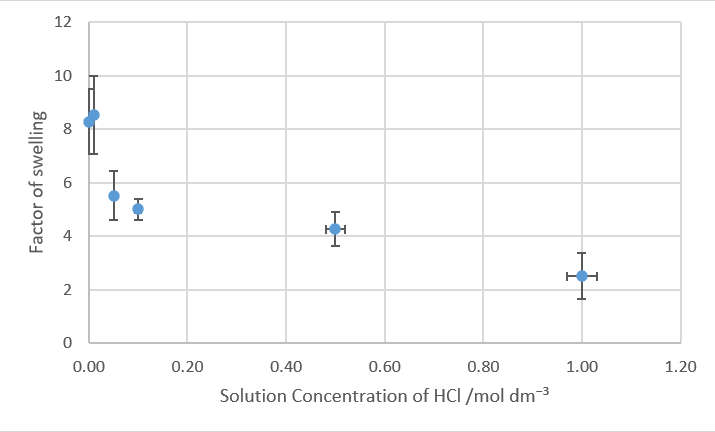
\includegraphics[width=\linewidth]{procDataRaw.png}
        \caption{Factor of swelling of bentonite clay as a function of \ce{[HCl]}}
        \label{fig:procDataRaw}
    \end{figure}
\end{paracol}

Plotting this processed data as Factor of swelling of bentonite clay as a function
of \ce{[HCl]} results in the graph in Figure \ref*{fig:procDataRaw}.

% \begin{figure}[H]
%     \centering
%     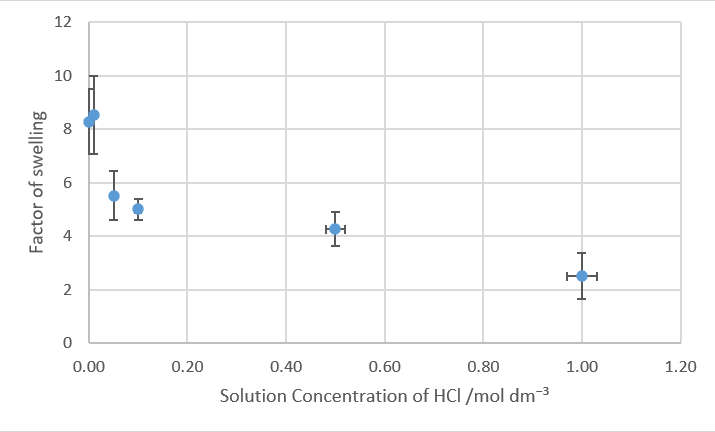
\includegraphics[width=0.5\textwidth]{procDataRaw.png}
%     \caption{Factor of swelling of bentonite clay as a function of \ce{[HCl]}}
%     \label{fig:procDataRaw}
% \end{figure}


Recall that the original hypothesis stated that the relationship between
the responding and manipulated variable is inversely proportional,
which is evident in the graphed data. However, the parts of the hypothesis
that aren't so evident in the experimental data is that
the relationship would initially be linear and then approach
a horizontal asymptote.

Given that the gradient change is very immediate at approximately \(\ce{[HCl]} = \SI{0.050}{mol.dm^{-3}}\)
as well as the maintenance of a lower gradient for a significantly wider domain
between \(\ce{[HCl]} = \SI{0.100}{mol.dm^{-3}}\) to \(\ce{[HCl]} = \SI{1.00}{mol.dm^{-3}}\),
the original section of the hypothesis regarding an initial linear relationship
transitioning to an asymptote has been proven to be false.

However, the possibility of the presence of a horizontal asymptote is not
removed. In hindsight of seeing the experimental relationship from the concentrations
of \ce{HCl} used in this experiment in that the final 3 data points maintain
a relatively steady curve that sit above a factor of swelling of 2,
it could be argued that since the minimum logical factor of swelling is 1, then the effects of an asymptote could have been observed had
the domain of concentrations of \ce{HCl} been significantly extended.

At a glance, the overall trend of the graph may either appear to be logarithmic,
exponential, or of a reciprocal function. However, a logarithmic relationship
does not have a horizontal asymptote, meaning that such a relationship would
not apply to this experiment as the swelling factor must approach a plateau
as \ce{Na+} ions are depleted.

Figures \ref*{fig:exponential} and \ref*{fig:reciprocal} present the
exponential and reciprocal best-fit trendline respectively.
Visually speaking, the reciprocal trendline has a signficantly
better fit than the exponential trendline. This is numerically
proven from the coefficients of determination (\(R^2\)) between the two
relationships, where the \(R^2\) value of the exponential best-fit trendline
is 0.7165 whereas the \(R^2\) value of the reciprocal best-fit trendline
is 0.9512.

\begin{multicols}{2}
    \begin{figure}[H]
        \centering
        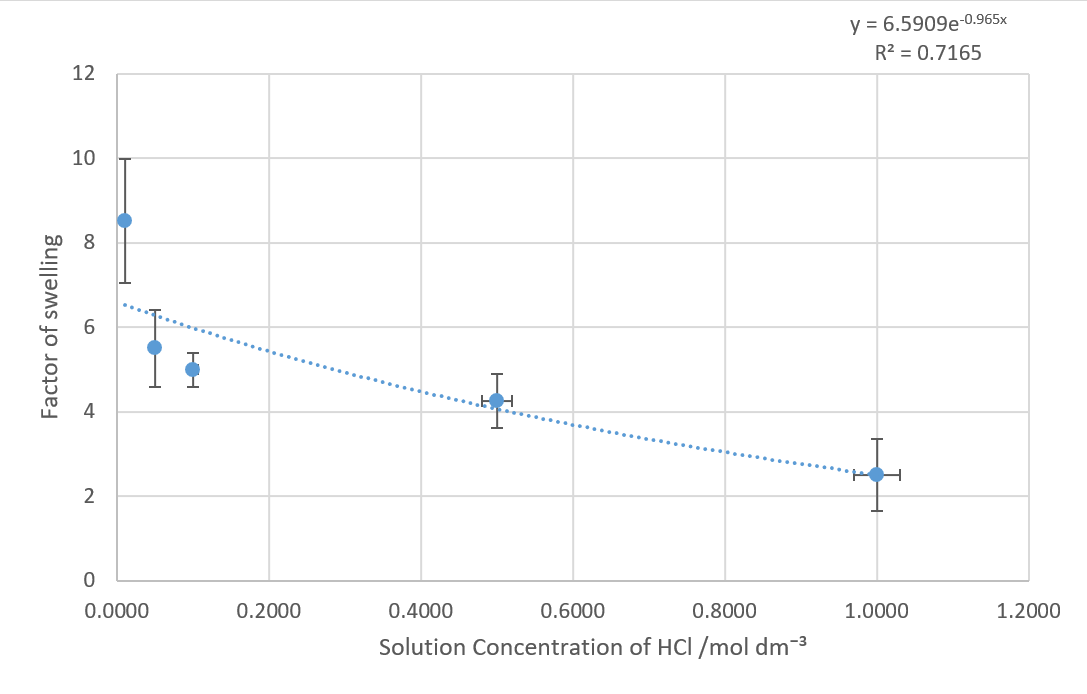
\includegraphics[width=\linewidth]{exponential.png}
        \caption{Factor of swelling of bentonite clay as a function of \ce{[HCl]} with an exponential trendline}
        \label{fig:exponential}
    \end{figure}
    \begin{figure}[H]
        \centering
        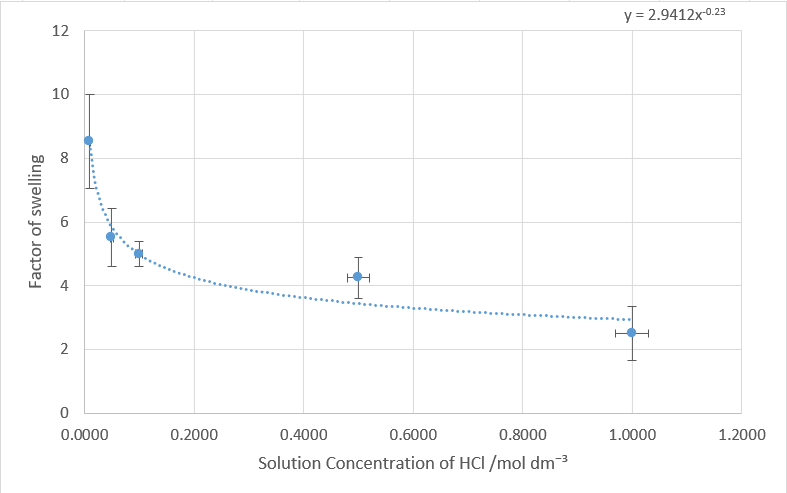
\includegraphics[width=0.9\linewidth]{reciprocal.png}
        \caption{Factor of swelling of bentonite clay as a function of \ce{[HCl]} with a reciprocal trendline}
        \label{fig:reciprocal}
    \end{figure}
\end{multicols}

\cite{ramavaraprasadSwellingCharacteristicsSoils2018a}
does not provide upfront any graphs for comparison under
the context of this investigation. However, there is enough
information within this source to analyze and convert
into something insightful under this investigation's context.
The final values of the swelling percentage in Figure \ref*{fig:literature} can
be taken to determine to graph swelling percentage as
a function of \ce{[H_3O+]} according to these literature
values.

Note that concentrations in the literature data are measured in
normality (\unit{N}), which is defined as
``the number of gram or mole equivalents of solute present in one litre of a solution'' \cite{Normality}.
Molarity can be determined from the
formula \(M = \frac{N}{n}\), where \(M\) is the molarity of the
acid /\unit{mol.dm^{-3}}, \(N\) is the normality of the solution
/\unit{N}, and \(n\) is the number of protons in the acid \cite{gonzalesHowCalculateNormality2017}.

Sample calculations for the conversions
from normality to molarity are shown below.

\begingroup
\allowdisplaybreaks
\begin{paracol}{2}
    \begin{align*}
         & N = \SI{4}{N}~ \ce{H_2SO_4},\quad n = 2
        \\
         & M = \frac{N}{n}
        \\
         & = \frac{\SI{4}{N}~ \ce{H_2SO_4}}{2}
        \\
         & = \SI{2}{mol.dm^{-3}}~ \ce{H_2SO_4}
        \\
         & \ce{[H_3O+]} = \SI{2}{mol.dm^{-3}}
    \end{align*}
    \switchcolumn
    \begin{align*}
         & N = \SI{4}{N}~ \ce{H_3PO_4},\quad n = 3
        \\
         & M = \frac{N}{n}
        \\
         & = \frac{\SI{4}{N}~ \ce{H_3PO_4}}{3}
        \\
         & = \SI{1.3}{mol.dm^{-3}}~ \ce{H_3PO_4}
        \\
         & \ce{[H_3O+]} = \sqrt{K_a \times \ce{[H_3PO_4]}}
        \\
         & = \sqrt{6.9 \times 10^{-3} \times \SI{1.3}{mol.dm^{-3}}}
        \\
         & = \SI{0.1}{mol.dm^{-3}}
    \end{align*}
\end{paracol}
\endgroup


\begin{paracol}{2}
    \begin{figure}[H]
        \centering
        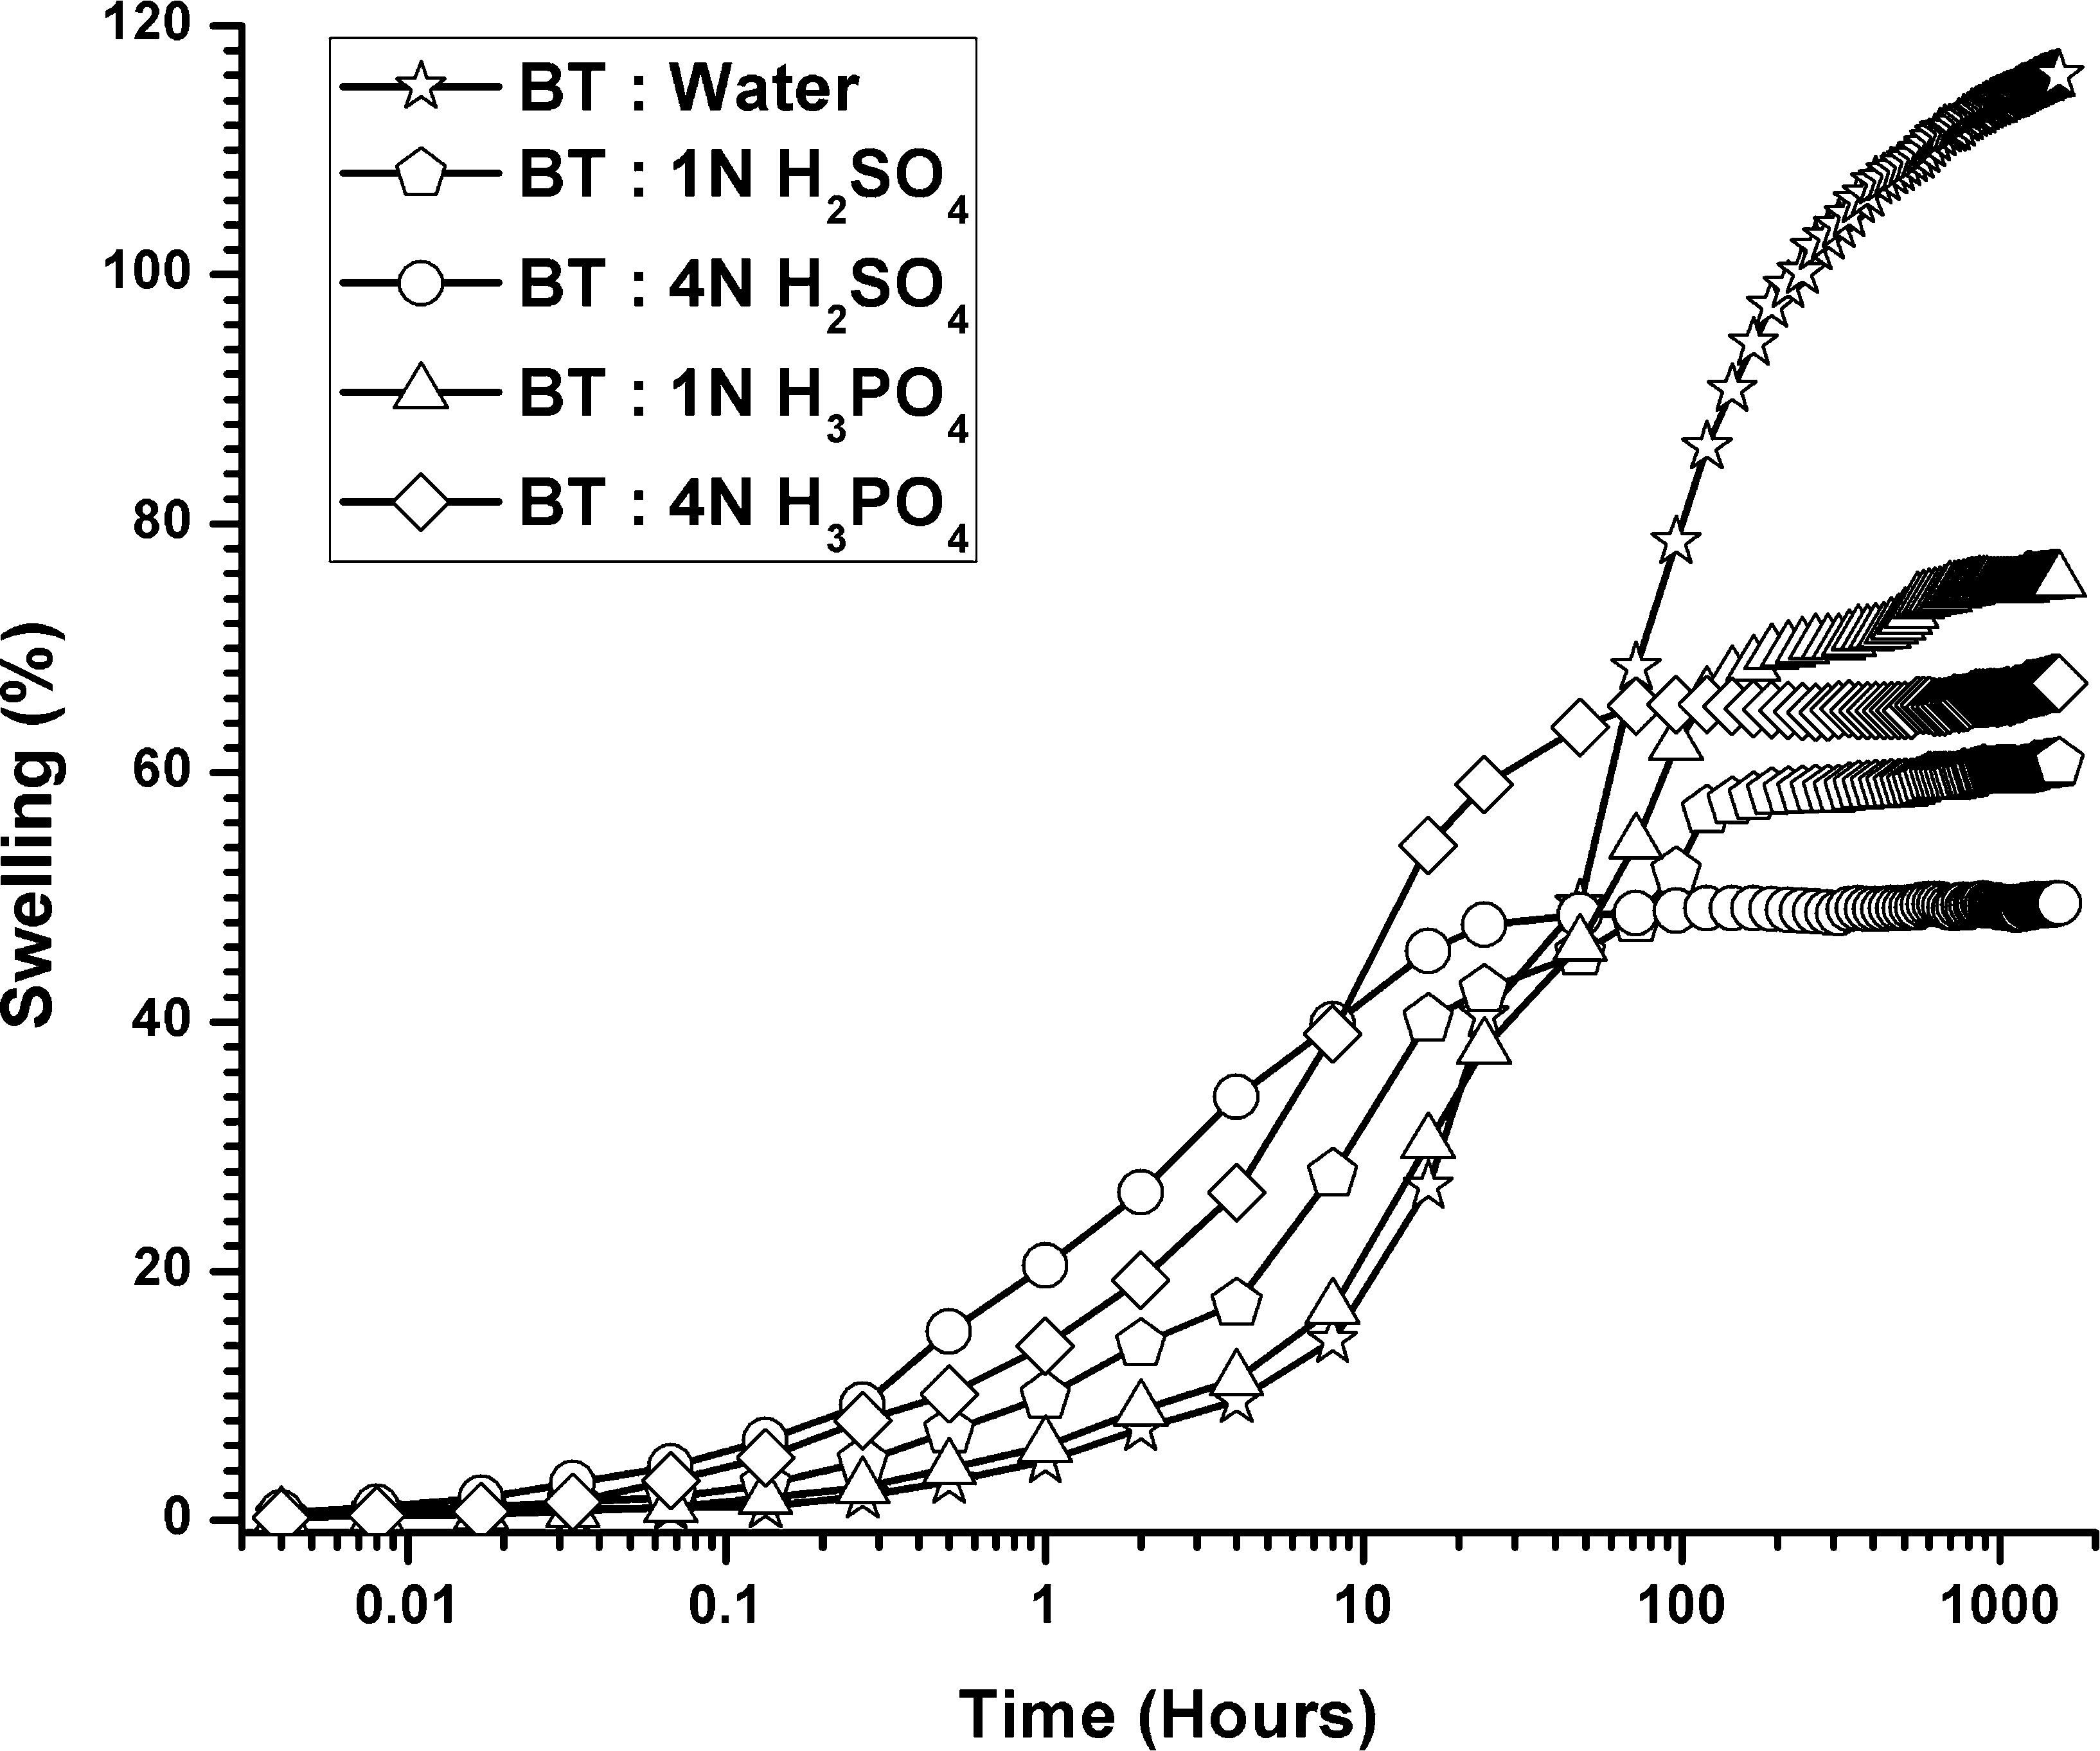
\includegraphics[width=0.7\linewidth]{literature.png}
        \caption{Literature data of Swelling percentage /\% as a function of Time /\unit{h} \protect\cite{ramavaraprasadSwellingCharacteristicsSoils2018a}}
        \label{fig:literature}
    \end{figure}
    \switchcolumn
    \begin{table}[H]
        \fontsize{9pt}{9pt}\selectfont
        \centering
        \caption{Literature values of final swelling percentage as a function of concentration of hydronium ions}
        \begin{tblr}{
            width = \linewidth,
            colspec = {Q[683]Q[260]},
            hlines,
            vlines,
            }
            Concentration of~$\ce{H_3O+}$~/$\unit{mol.dm^{-3}}$ & Swelling Percentage /\% \\
            2                                                   & 50                      \\
            0.5                                                 & 60                      \\
            0.1                                                 & 68                      \\
            0.05                                                & 76                      \\
            0                                                   & 116
        \end{tblr}
    \end{table}

\end{paracol}

Graphing the literature data produces the graph in Figure \ref*{fig:procLiterature},
which further confirms the hypothesis that factor of swelling
is inversely proportional to \ce{[H+]}.

\begin{paracol}{2}
    \begin{figure}[H]
        \centering
        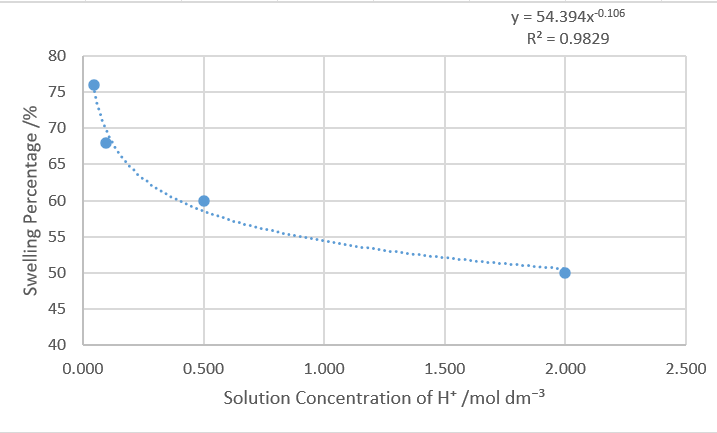
\includegraphics[width=\linewidth]{procLiterature.png}
        \caption{Swelling percentage /\% as a function of concentration of \ce{H+} ions in solution from literature data \protect\cite{ramavaraprasadSwellingCharacteristicsSoils2018a}}
        \label{fig:procLiterature}
    \end{figure}
    \switchcolumn
    \begin{figure}[H]
        \centering
        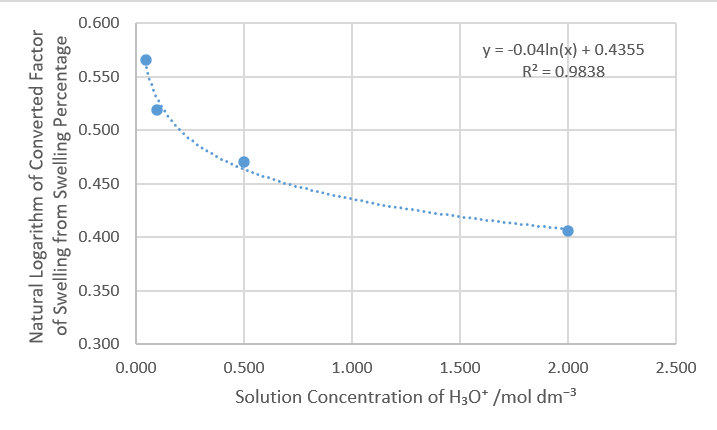
\includegraphics[width=\linewidth]{lnLiterature.png}
        \caption{Natural logarithm of factor of swelling converted from swelling percentage as a function of concentration of \ce{H+} ions in solution from literature data \protect\cite{ramavaraprasadSwellingCharacteristicsSoils2018a}}
        \label{fig:lnLiterature}
    \end{figure}
\end{paracol}

To thoroughly compare this experiment's results against the literature
data, it is best to find a way to linearize both relationships.
If a reciprocal relationship is the best-fit for the relationship,
then an idea from kinetics for linearization is to reciprocate
the factor of swelling or swelling percentage. While doing
this with the experimental data yield a result that is possibly
linear as seen in Figure \ref*{fig:reciprocalLinearization}, doing this with the literature data yields a result
that is not linear as seen in Figure \ref*{fig:reciprocalLiterature}.
Taking the natural logarithm of the dependent variable was also
a linearization technique from kinetics; however, this also fails
to produce a linear relationship as seen in Figure \ref*{fig:lnLiterature}.

\begin{paracol}{2}
    \begin{figure}[H]
        \centering
        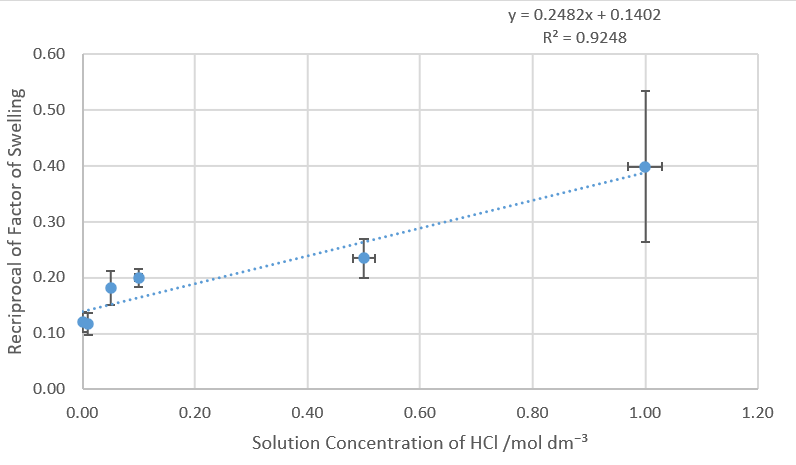
\includegraphics[width=\linewidth]{reciprocalLinearization.png}
        \caption{Reciprocal of factor of swelling as a function of [\ce{HCl}] from experimental data}
        \label{fig:reciprocalLinearization}
    \end{figure}
    \switchcolumn
    \begin{figure}[H]
        \centering
        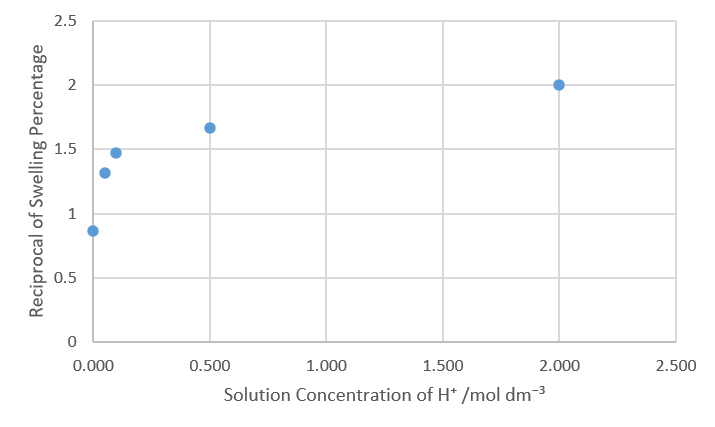
\includegraphics[width=\linewidth]{reciprocalLiterature.png}
        \caption{Reciprocal of swelling percentage as a function of [\ce{H+}] from literature data \protect\cite{ramavaraprasadSwellingCharacteristicsSoils2018a}}
        \label{fig:reciprocalLiterature}
    \end{figure}
\end{paracol}


The method that produces the best linear results for both the experimental and literature data is by graphing
the swelling factor or swelling percentage as a function of
the pH of the acidic solution. Figure \ref*{fig:experimentalPH} shows this with the experimental
data, and Figure \ref*{fig:literaturePH} shows this with the literature data.
\textit{Note that this relationship is not entirely linear in either of the
    two graphs and the presence of the linear trendline is to identify these subtleties
    in the evaluation}.

\begin{paracol}{2}
    \begin{figure}[H]
        \centering
        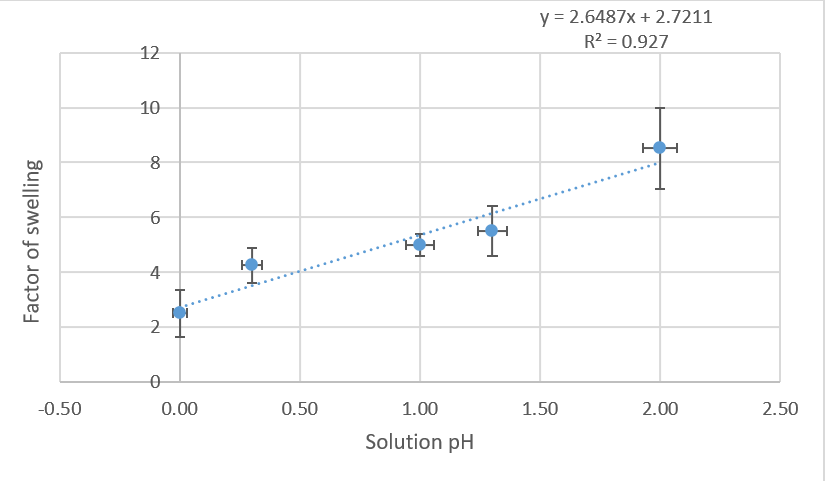
\includegraphics[width=\linewidth]{experimentalPH.png}
        \caption{Factor of swelling as a function of solution pH from experimental data}
        \label{fig:experimentalPH}
    \end{figure}
    \switchcolumn
    \begin{figure}[H]
        \centering
        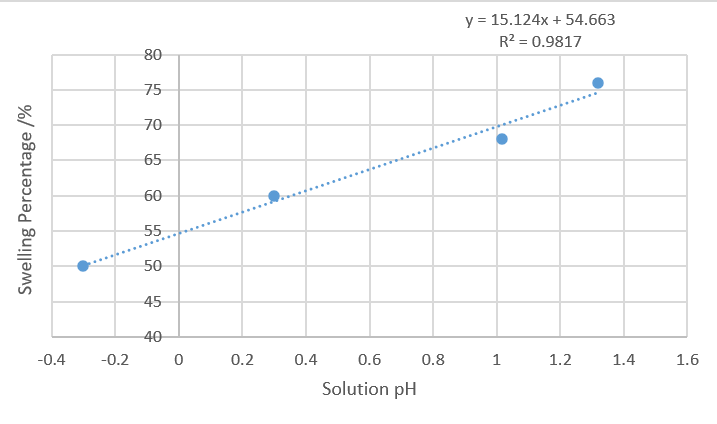
\includegraphics[width=\linewidth]{literaturePH.png}
        \caption{Swelling percentage /\% as a function of solution pH from literature data \protect\cite{ramavaraprasadSwellingCharacteristicsSoils2018a}}
        \label{fig:literaturePH}
    \end{figure}
\end{paracol}

\section{Conclusion}

\subsection{Summary}

Contrary to the hypothesis, the experimentally determined relationship
between the factor by which the sodium bentonite clay swells
and the concentration of \ce{H+} ions of an acidic solution /\unit{mol.dm^{-3}}
when the acidic solution and bentonite mix is inversely proportional, specifically
of a reciprocal relationship (\(F \propto \frac{1}{\ce{[HCl]}}\)).

% With reference to Figures \ref*{fig:experimentalPH} and \ref*{fig:literaturePH},
% the experimental data matches the literature data in terms of
% the subtle trend in the data points, where in both graphs,
% data points around when pH is 0.3 is above the trendline
% and data points around when pH is 1 is below the trendline.

Upon closer comparison between the experimental data in Figure \ref*{fig:reciprocalLinearization}
and the literature data in Figure \ref*{fig:reciprocalLiterature},
one will notice that the two graphs do follow a similar trend
until when \(\ce{[HCl]} = \SI{1.00}{mol.dm^{-3}}\) in the
experimental data where the trend is broken. This indicates
that the experimental data point for when \(\ce{[HCl]} = \SI{1.00}{mol.dm^{-3}}\)
is not reliable, specifically that it is lower than reality.

Considering both \(pH = -\log [\ce{H+}]\) and \(F \propto \frac{1}{\ce{[HCl]}}\),
the mathematical prediction would be that factor of swelling as a
function of pH would be an exponential function. This confirms
that Figure \ref*{fig:experimentalPH} is not linear, with
the factor of swelling at pH = 0 (\(\ce{HCl} = \SI{1.00}{mol.dm^{-3}}\))
previously proven to be an outlier. The linear appearance of the literature
data in Figure \ref*{fig:literaturePH} is likely due to its
restricted domain, as substantial change in gradient
of Figure \ref*{fig:experimentalPH} isn't observed
until \(\ce{[H+]} > 1.50\), which the literature data does not
exceed this pH value.

Ultimately, while this investigation disproved the hypothesis
by demonstrating an inversely proportional relationship between
the factor of swelling and the concentration of \ce{HCl} in the
mixed solution, the data did not lead to a precise and
background-based mathematical relationship between the
two variables.

\subsection{Evaluation}

\begin{table}[H]
    \centering
    \begin{tblr}{
        width = \linewidth,
        colspec = {Q[110]Q[298]Q[292]Q[240]},
        hlines,
        vlines,
        }
        Source of Error                                                                                             & Effect on data                                                                                                                                                                                                                                                                                                                                 & Effect on result                       & How might this error be corrected in a future experiment                                                                   \\
        High ratio of solution to clay                                                                              & {Uncertainty of the~$\SI{10}{mL}$~graduated cylinder is significant in comparison to the final volumes of the bentonite clay.                                                                                                                                                                                                                                                                                                                                                                                        \\Any volumes that were below the minimum graduation were not accurate.} & {Large final uncertainties in the factor of swelling\\Any concentrations of~$\ce{HCl}$ that lead to the final volume to be lower than the minimum graduated cylinder graduation are deemed unreliable. In this investigation, it was when~$\ce{[HCl]} = \SI{1.00}{mol.dm^{-3}}$~and caused the final factor of swelling for that concentration to be lower than reality.} & Determining a ratio that offers enough use of bentonite clay to make the graduated cylinder's uncertainty insignificant that does not lead to overflow of clay or solution during swelling nor lead to irregular distribution of absorption throughout the clay\\
        Loss of bentonite clay during transfer to graduated cylinder due to stickiness to glassware and weigh boats & {Losing bentonite in the process of transferring it to the graduated cylinder would cause the amount of bentonite mixed within the solution to be less than $\SI{1.00}{mL}$. This in turn would cause the final volume of swollen bentonite to be lower than reality, potentially in multiples relative to the original loss of dry bentonite.                                                                                                                                                                       \\Because the amount of bentonite lost between each trial will vary, this source of error also contributes to variability in the final volume of submerged bentonite clay.} & {Lower factor of swelling than reality.\\Contributes to variability on the factor of swelling.} & Scratch as much of the remaining bentonite on each weigh boat and perform another round of transferring bentonite to each graduated cylinder. Take each graduated cylinder and tilt it to a degree such that any bentonite stuck on the upper portion of the graduated cylinder is removed.\\
        Significant portion of bentonite being in the form of large granules                                        & The true volume of bentonite standardized to mass is lower than~$\SI{1.0}{mL}$. This would also mean that the volume of bentonite mixed with the solutions is lower than reality, causing the final volume of swollen bentonite to be lower than reality.                                                                                      & Lower factor of swelling than reality. & Incorporate into the process a section dedicated to pulverizing the bentonite. This can be done using a mortar and pestle.
    \end{tblr}
\end{table}

Despite these sources of error, the methodology and process in this
investigation allows for simple experimentation surrounding
clay swelling. Overall, omitting the last experimental data point
when \(\ce{[HCl]} = \SI{1.00}{mol.dm^{-3}}\), the trend of the
data points fit very similarly to the literature data. This
is despite that fact that this experiment was performed
using common laboratory equipment instead of scarce
equipment dedicated for these types of investigations.

\section{Extension}

Another area of investigation regarding clay soil swelling
is determining the relationship between factor of swelling
and the surface area to volume ratio of the clay soil.
The soil can be separated according to their
size using sieves of various aperture sizes, which
will indicate the diameter of the filtered clay.


\bibliographystyle{apacite}
\bibliography{IB_CHEM_IA.bib}

\end{document}